\documentclass{scrbook}
\usepackage{graphicx} % Required for inserting images
\usepackage{tabularx} % Required for fixed width tables
\usepackage{adjustbox} % Required to put images inside tables
\usepackage{scrlayer-scrpage} % Required for the subtitles
\usepackage{url} % Required for the URLs
\usepackage{hyperref} % Required for the URLs


\title{Distributed and transactional systems}
\subtitle{Ambient intelligence course (A.Y. 2025/2026)\\Topic taught by Prof. Floriano Scioscia}
\author{Gabriele Colapinto}
\date{\today}

\begin{document}

\maketitle
\thispagestyle{empty}

{\Large\textbf{License}} \\
{Notes from Ambient intelligence (A.Y. 2025/2026) by Gabriele Colapinto. 
Course taught by professors Michele Ruta, Floriano Scioscia, Arnaldo Tomasino, Davide Loconte — 
Licensed under CC BY-NC 4.0.\\
\url{https://creativecommons.org/licenses/by-nc/4.0/}}

\vspace*{\fill}
\rule{\textwidth}{0.2pt}
\small{© 2025 Gabriele Colapinto \\
Released under the \href{https://creativecommons.org/licenses/by-nc/4.0/}{Creative Commons Attribution–NonCommercial 4.0 International License}}

\clearpage

\tableofcontents

\chapter{Introduction to Distributed Systems}


A distributed information system is formally defined as a collection of
modules that run concurrently on independent, interconnected computers.
The strategic importance of understanding these systems lies in their
prevalence in the architecture of modern computing, from hyperscale
cloud infrastructure to globally distributed Internet of Things (IoT)
ecosystems. Each individual module that participates and cooperates
within the system is generically referred to as a~\textbf{node}.

The fundamental nature of a distributed system is defined by three core
characteristics:

\begin{itemize}
\item
  \textbf{Concurrent Operation:}~All modules within the system are
  "alive at the same time." They operate in parallel and must interact
  with one another to perform the system\textquotesingle s overall
  function.
\item
  \textbf{Independent Devices:}~There is no single, central
  administrative computer that controls all the modules. Each node runs
  on a separate device that can be started, shut down, or changed
  independently of the others.
\item
  \textbf{Interconnectivity:}~The independent nodes are connected via a
  computer network, which allows them to exchange information and
  coordinate their actions.
\end{itemize}

For these independent, concurrent nodes to cooperate effectively, they
must adhere to common interoperability standards that govern how they
communicate.

\section{Interoperability: Enabling Communication Between
Nodes}

\subsection{The Challenge of Interoperability}

Interoperability is a critical requirement for any distributed system,
as it enables the constituent nodes to communicate and work together.
The mechanism chosen to define the interface between nodes has profound
implications for the system\textquotesingle s flexibility,
maintainability, and the degree of coupling between its components.
Historically, the evolution from tightly-coupled to loosely-coupled
interfaces was not merely an academic exercise; it was driven by the
practical necessities of building massively scaled, heterogeneous
systems like the World Wide Web. Two primary approaches to designing
these interfaces have emerged: API-based and protocol-based.

\subsubsection{API-based (RPC)}

\textbf{Mechanism:}~This model is based on providing an Application
Programming Interface (API) that typically uses Remote Procedure Calls
(RPC). One node can directly invoke a procedure or method on a remote
node as if it were a local function call.

\textbf{Historical Context:}~This is an earlier approach in computer
science, with its origins in the 1980s.

\textbf{Primary Drawback:}~This approach creates~\textbf{tight
coupling}. If significant changes are made to a module\textquotesingle s
API, the implementation of all other modules that call it must also be
modified, making the system rigid and difficult to maintain.

\subsubsection{Protocol-based}

\textbf{Mechanism:}~Nodes interact using standardized communication
protocols and data interchange formats. This approach defines the rules
of engagement rather than exposing internal functions directly.

\textbf{Key Advantage:}~Enables superior decoupling between nodes. As
long as the protocol contract is honored, the internal implementation of
a node can be modified without impacting other nodes in the system.

\textbf{Protocol Components:}~A protocol specifies:~\\
• The operational~\textbf{states}~a node can be in.~\\
• The~\textbf{messages}~(with defined types and structures) that can be
exchanged.~\\
• The~\textbf{rules}~governing how a node transitions from one state to
another based on the messages it sends or receives.

\subsubsection{Conclusions}

This fundamental choice of interface---tightly-coupled RPC or
loosely-coupled protocol---constrains and informs the subsequent
selection of a communication model for message exchange.

\subsection{Core Communication Models: Synchronous vs. Asynchronous}

\subsubsection{Analyzing Communication Patterns}

Beyond the type of interface, the communication~\emph{model}~determines
how nodes exchange information, which directly impacts system
performance, resource utilization, and overall design complexity. The
primary distinction is between blocking (synchronous) and non-blocking
(asynchronous) models of communication.

\subsubsection{Synchronous (Blocking) Communication}

\begin{figure}[h]
    \centering
    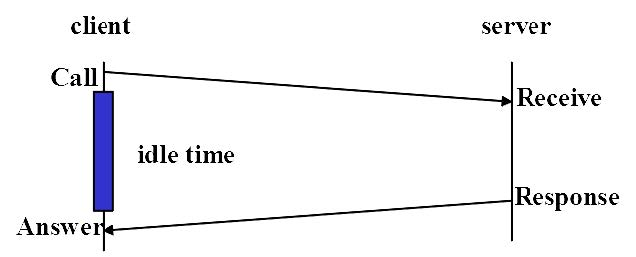
\includegraphics[width=0.8\textwidth]{Images/Synchronous_communication.jpg}
    \caption{Synchronous communication}
\end{figure}

Synchronous communication is a blocking model where a node, after
sending a message or calling a remote procedure, halts its own
operations and waits idly for a response to arrive.

The trade-offs of this model are straightforward:

\begin{itemize}
\item
  \textbf{Advantage:}~It is conceptually simpler and therefore easier to
  design and implement. The program flow is linear and more predictable.
\item
  \textbf{Disadvantage:}~It wastes resources and creates significant
  performance bottlenecks. The time the calling node spends waiting is
  "idle time" during which it could be performing other useful work.
\end{itemize}

\subsubsection{Asynchronous (Non-Blocking) Communication}

\begin{figure}[h]
    \centering
    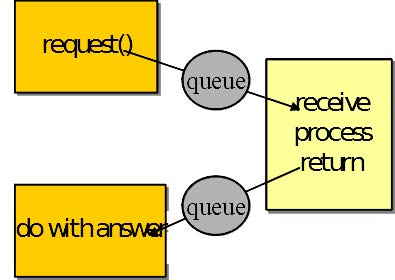
\includegraphics[width=0.6\textwidth]{Images/Asynchronous_communication.jpg}
    \caption{Asynchronous communication}
\end{figure}

Asynchronous communication is a non-blocking model designed to improve
performance and increase decoupling between nodes. Instead of waiting, a
node can send a message and continue with other tasks. Several patterns
enable this model:

1.~\textbf{Queue-based:}~Each node possesses a dedicated queue for
incoming messages. A sending node simply adds a message to the
recipient\textquotesingle s queue. The receiving node can then
accumulate requests from multiple sources and process them at its own
pace, decoupling the sender\textquotesingle s timing from its own.

2.~\textbf{Event-based:}~Communication is triggered by the occurrence of
specific "events." These events can represent a change in a
node\textquotesingle s internal state, an external action from a user,
or a change in an environmental parameter, such as a sensor reading
crossing a predefined threshold.

3.~\textbf{Topic-based (Publish-Subscribe):}~This is a powerful
generalization where each node can maintain several message queues, with
each queue being associated with a specific "topic." Nodes can
"subscribe" to a topic, effectively creating a dedicated queue for it.
Another node can then "publish" a message to that topic, and the system
ensures all subscribing nodes receive it, enabling a highly decoupled,
one-to-many communication pattern.

While the asynchronous approach leads to better performance and
architectural decoupling, it introduces its own set of trade-offs. It is
considerably harder to design and implement, as developers must manage
non-linear program flows and potential race conditions. It also requires
more memory and processing resources to manage queues and
message-handling logic. Furthermore, this model necessitates more
sophisticated protocols. Because a computer network is inherently
unreliable---that is, when data is sent, its arrival is not
guaranteed---asynchronous systems require protocols that provide message
delivery guarantees to prevent data loss. The choice of a communication
model is therefore a foundational decision that shapes the
system\textquotesingle s architecture.

\chapter{Architectural Paradigms: Client-Server and
Peer-to-Peer}

\begin{figure}[h]
    \centering
    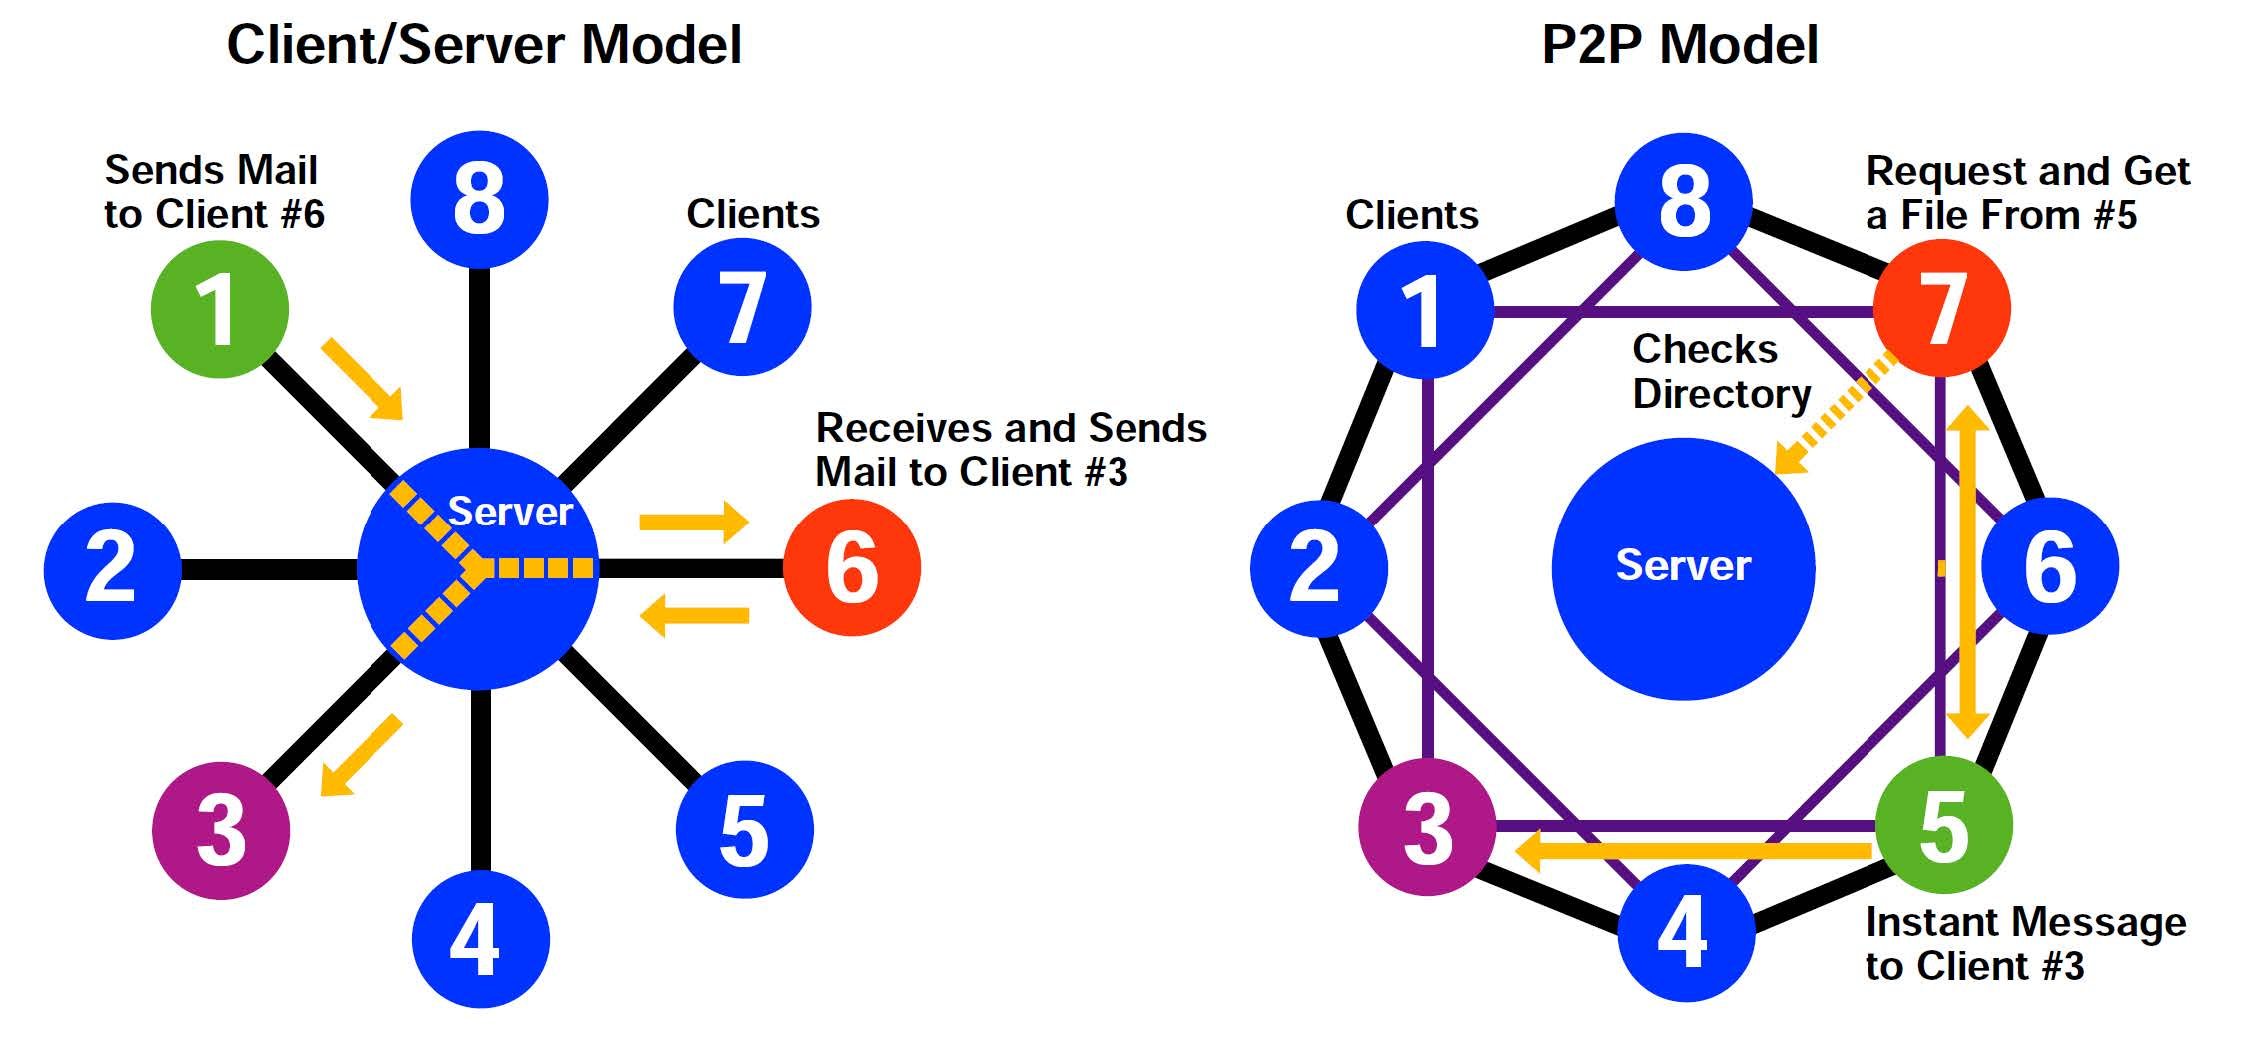
\includegraphics[width=0.6\textwidth]{Images/Client_server_P2P.jpg}
    \caption{Client-Server and P2P models}
\end{figure}

\section{Structuring the Distributed System}

Distributed systems are generally organized according to one of two
major architectural paradigms: client-server or peer-to-peer (P2P). This
architectural choice is fundamental, as it defines the roles of the
nodes within the system, the distribution of resources, and the overall
flow of information.

\subsection{The Client-Server Model}

In a client-server architecture, nodes assume one of two distinct
roles.~\textbf{Clients}~are nodes that make requests for data or
services.~\textbf{Servers}~are nodes that receive these requests,
process them, and provide responses back to the clients.

This architecture is typically characterized by an imbalance: there are
far more clients than servers. Consequently, servers are generally more
powerful nodes, equipped with greater memory, processing power, and
network bandwidth to handle concurrent requests from numerous clients. A
simple, single-threaded server that can only handle one client at a time
is often inadequate. To manage high loads, servers require more complex
internal designs, such as being~\textbf{multi-threaded}~to process
multiple requests in parallel. A common advanced pattern involves
deploying servers in a~\textbf{cluster}~managed by a~\textbf{load
balancer}. This load balancer acts as a facade; it receives all incoming
requests and forwards each one to a different server instance, a process
which is entirely transparent to the clients.

\subsection{The Peer-to-Peer (P2P) Model}

The peer-to-peer model represents a fundamental shift in architectural
philosophy. In a P2P architecture, all nodes are
homogeneous~\textbf{peers}. Each peer is capable of acting as both a
client (making requests) and a server (providing responses).

The core idea of the P2P model is to move computing power and
information storage to the~\textbf{edge of the network}, where the
individual users reside. Historically, the~\textbf{first P2P
infrastructure}~was ARPANET in 1969, which was designed to be a
resilient network without a single point of failure. However, the term
"P2P" was popularized by the file-sharing application Napster in 1999,
which brought the technology to general public attention. This paradigm
eliminates the reliance on a few powerful, central servers and instead
leverages the collective resources of all participating nodes. The
structure of these networks, however, can vary significantly.

\section{A Deeper Analysis of Peer-to-Peer Architectures}

\subsection{The Bootstrapping Challenge in P2P Networks}

The primary operational challenge in any P2P network is~\textbf{network
bootstrapping}. This is the process through which a new peer, upon
starting up, discovers and connects to other existing peers to
successfully join the network. Without a reliable bootstrapping
mechanism, a new node would be isolated and unable to participate.

\subsection{Contrasting P2P Implementations}

To address the bootstrapping challenge and other design goals, P2P
networks are typically implemented using either a hybrid or a pure
architecture (See table 2.1).

\begin{table}
    \centering
    \begin{tabularx}{\textwidth}{|X|X|}
        \hline
        \textbf{Hybrid P2P} & \textbf{Pure P2P} \\ \hline
        \textbf{Mechanism:}~This architecture includes a special, central
        node---variously known as a~\textbf{tracker}, director, or bootstrapping
        node---whose job is to facilitate peer discovery. &
        \textbf{Mechanism:}~This architecture does not use any central server or
        tracker. All nodes are functionally identical, and discovery must be
        handled in a fully decentralized manner. \\ \hline
        \textbf{Bootstrapping Process:}~A new peer, using the pre-configured,
        fixed network address of the tracker, requests a list of active peers to
        connect with. & \textbf{Bootstrapping Process:}~Bootstrapping is more
        difficult, as peers must locate each other without relying on a central
        director. \\ \hline
        \textbf{Key Liability:}~The central tracker represents a~\textbf{single
        point of failure}. If the tracker goes offline, new peers cannot join
        the network, and the system\textquotesingle s ability to grow or recover
        is severely compromised. & \textbf{Key Advantage:}~By eliminating the
        central node, this model avoids the risk of a single point of failure,
        which significantly increases the overall resilience and fault tolerance
        of the system. \\ \hline
    \end{tabularx}
    \caption{Hybrid P2P and Pure P2P architectures}
\end{table}

\subsubsection{Case Study: The ROS Master as a Tracker
Analogy}\label{case-study-the-ros-master-as-a-tracker-analogy}

A clear, practical analogy for the hybrid P2P model can be found in the
Robot Operating System (ROS). In a ROS system, the~\textbf{ROS
Master}~functions almost exactly like a P2P tracker. It acts as a
central name server that allows different software components (nodes) to
register their existence and discover one another.

Crucially, the ROS Master does not handle the actual data exchange
between nodes. Once a subscriber node queries the Master and discovers
the location (IP address and port) of a publisher node, the two nodes
establish a direct peer-to-peer connection to exchange messages. This
illustrates a powerful and recurring pattern in distributed systems:
leveraging a centralized service for discovery and bootstrapping to
enable fully decentralized, high-performance interaction, thereby
balancing operational simplicity with scalable performance.

\subsection{Defining the Peer-to-Peer (P2P)
Architecture}\label{defining-the-peer-to-peer-p2p-architecture}

\begin{figure}[h]
    \centering
    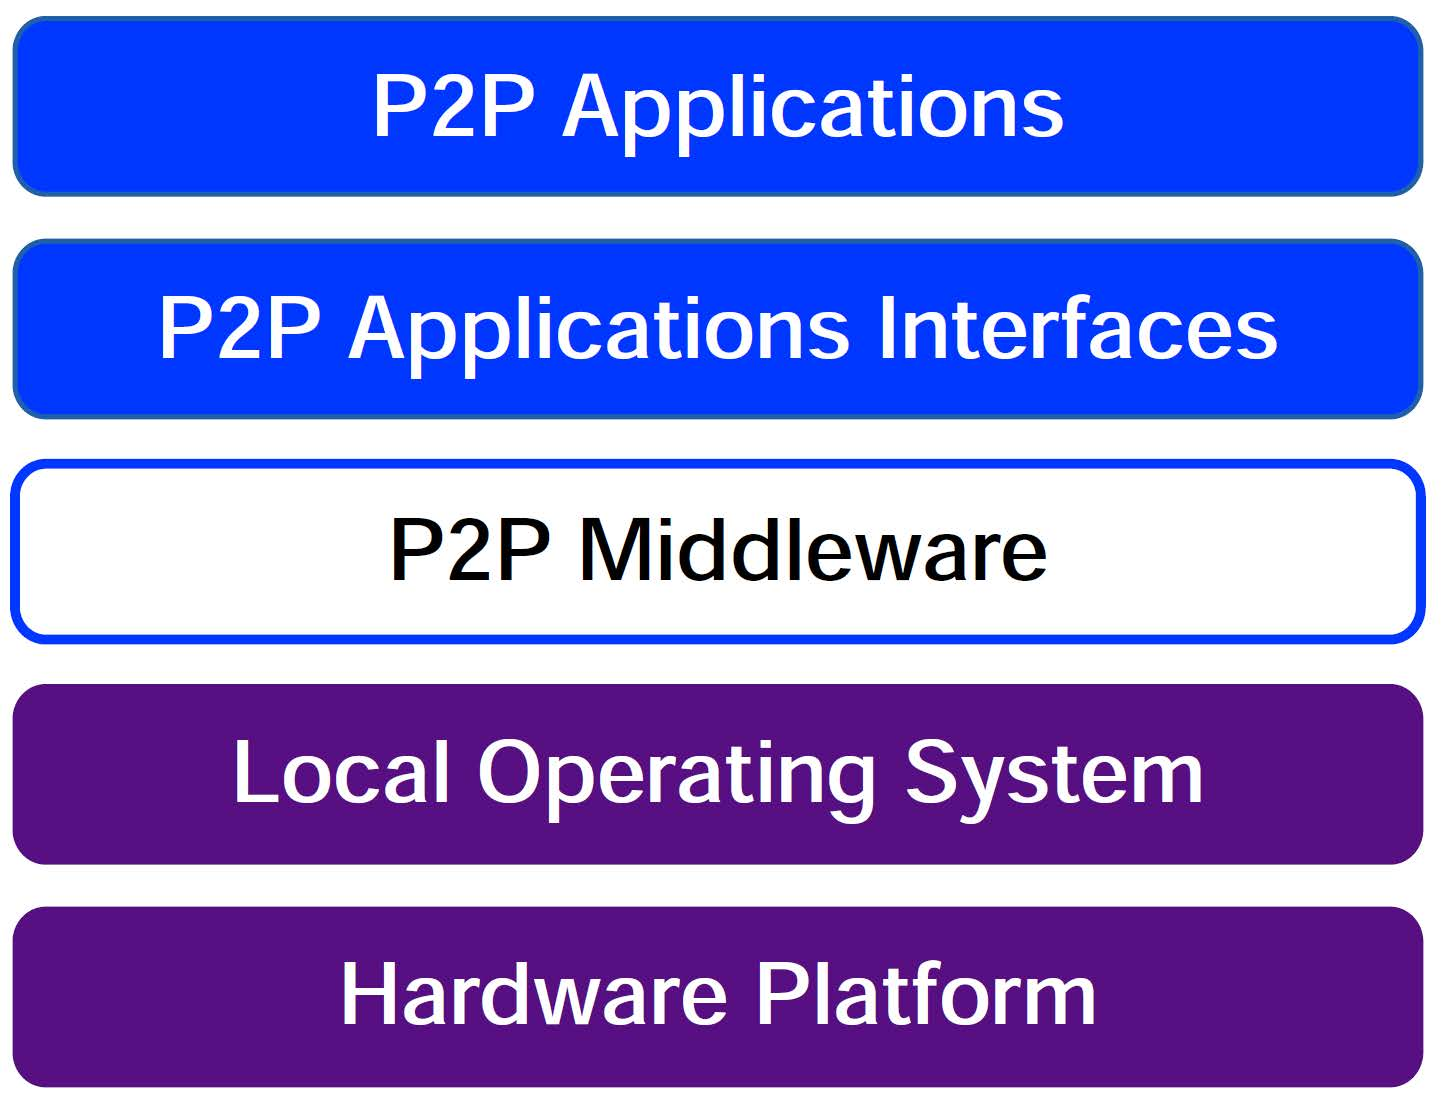
\includegraphics[width=0.6\textwidth]{Images/P2P_Stack.jpg}
    \caption{P2P stack}
\end{figure}

Peer-to-Peer (P2P) architecture is a decentralized computing model in
which network participants, known as~\textbf{peers}, share resources
directly with each other without the need for a central server. In this
model, each node acts as both a client and a server, contributing to the
collective power of the network for tasks such as data sharing and
computation.

This functionality is enabled by~\textbf{P2P middleware}, a software
layer that performs a set of general functions essential for network
operation. These core functions include:

\begin{itemize}
\item
  Allowing a new peer to~\textbf{join}~the network.
\item
  Enabling a peer to~\textbf{expose}~its local resources to other
  participants.
\item
  Facilitating the~\textbf{discovery}~of resources shared by other peers
  across the network.
\end{itemize}

The versatility of this model has led to its adoption across a wide
range of applications, which can be broadly categorized as follows:

\begin{itemize}
\item
  \textbf{Content Sharing:}~Primarily known for file sharing (e.g.,
  Napster, Gnutella), but also used for streaming and web conferencing.
\item
  \textbf{Hardware Resource Sharing:}~Leveraging the collective
  computing cycles of peers for distributed computation (e.g.,
  SETI@home).
\item
  \textbf{Communication:}~Powering instant messaging, conferencing, and
  other real-time communication platforms (e.g., Skype).
\item
  \textbf{Collaboration:}~Creating environments where peers can work
  jointly on shared resources.
\end{itemize}

\subsection{Comparing P2P with Other Distributed System
Models}\label{comparing-p2p-with-other-distributed-system-models}

P2P computing is one of several models for distributed systems, each
with distinct characteristics and goals. Understanding these differences
is crucial for appreciating the unique position of the P2P paradigm.

\begin{itemize}
    \item
      \textbf{Cluster Computing}\\
      Cluster computing typically involves a set of~\textbf{homogeneous
      nodes}~(computers with similar hardware and operating systems)
      connected within a local network. The entire cluster is managed by
      a~\textbf{single authority}, which administers the distribution of
      jobs and resources.
    \item
      \textbf{Grid Computing}\\
      The conceptual goal of Grid computing is to make distributed       computational resources available as transparently as an electrical grid. Its technical characteristics include:~
    
          \begin{itemize}
          \item
            \textbf{Fine-grained resource description}, detailing hardware, software, and dynamic load status.~
          \item
            \textbf{Advanced matchmaking}~to pair specific job requirements with the best available resources.~
          \item
            \textbf{Resource utilization metering}~to track usage for payment or in kind exchanges.~Its primary adoption has been in academic and research settings for sharing large or specialized scientific equipment.
          \end{itemize}
          
    \item
      \textbf{Peer-to-Peer Computing}\\
      P2P computing connects independent and~\textbf{heterogeneous
      nodes}~that can belong to different individuals or organizations. It employs~\textbf{simpler and more scalable protocols}~for resource discovery and allocation compared to Grid computing. This simplicity and scalability for massive networks have led to its~\textbf{mass adoption}~in a wide variety of commercial and non-commercial applications.
\end{itemize}

It is also important to distinguish these models from~\textbf{Cloud
Computing}. While Cloud Computing inherited key technologies from Grid
computing, such as resource metering, it fundamentally relies on
a~\textbf{client-server model}, where a few large providers offer
resources to a vast number of clients.

\subsection{Analyzing the Core Benefits and Challenges of
P2P}\label{analyzing-the-core-benefits-and-challenges-of-p2p}

The decentralized nature of P2P architecture provides significant
advantages but also introduces a unique set of complex challenges.

\subsubsection{Benefits}

\begin{itemize}
\item
  \textbf{Avoidance of Bottlenecks:}~By eliminating central servers, P2P
  networks avoid the performance bottlenecks and single points of
  failure inherent in client-server systems.
\item
  \textbf{Resilience and Scalability:}~The decentralized structure
  enhances the system\textquotesingle s ability to handle load spikes
  and continue functioning even if some nodes fail or leave the network.
\item
  \textbf{Robustness Against Attacks:}~Pure P2P networks are highly
  robust against denial-of-service (DoS) attacks, as there is no single
  target to incapacitate the entire system.
\item
  \textbf{Low Deployment Cost:}~P2P networks can be deployed at a very
  low cost, as they leverage the existing hardware and resources of
  their participants.
\end{itemize}

\subsubsection{Challenges}

\begin{itemize}
\item
  \textbf{Cross-Platform Interoperability:}~Ensuring that middleware is
  compatible across diverse hardware and software platforms is a
  significant development hurdle.
\item
  \textbf{Network Complexities:}~P2P systems must effectively navigate
  common internet complexities such as firewalls, Network Address
  Translation (NAT), and dynamic IP addresses.
\item
  \textbf{Dynamic Nature of Peers:}~Peers can join and leave the network
  at any time without notice. Guaranteeing the continuous availability
  of resources in such a fluid environment requires mechanisms like data
  redundancy.
\item
  \textbf{Efficient Resource Discovery:}~Locating a specific resource in
  a large, decentralized network of independent nodes without a central
  index is a non-trivial problem.
\item
  \textbf{Security and Trust:}~Granting local autonomy to peers makes it
  difficult to prevent malicious behavior. Establishing trust among
  unknown and autonomous participants is a fundamental challenge,
  especially for critical applications.
\end{itemize}

These challenges, particularly the need for~\emph{efficient resource
discovery}~without a central index and~\emph{robustness}~against the
dynamic nature of peers, drove the evolution from simple unstructured
networks to the sophisticated structured systems we will now examine.

\subsection{Understanding P2P Network
Topology}\label{understanding-p2p-network-topology}

The topology of a P2P network---the way its nodes are
interconnected---is a critical factor that determines its performance,
resilience, and efficiency. In network science, topologies are modeled
as graphs, and various mathematical models can be used to describe their
structure and predict their behavior.

A network graph consists of~\textbf{vertices}~(the nodes or peers)
and~\textbf{edges}~that represent the communication links between them.
The~\textbf{degree}~of a node is the number of links it has to other
nodes. A graph where every node has the same degree is known as
a~\textbf{regular graph}. For instance, in a 3-regular graph, every
single node is connected to exactly three other nodes.

\subsubsection{Random Network Models}

\begin{figure}[h]
    \centering
    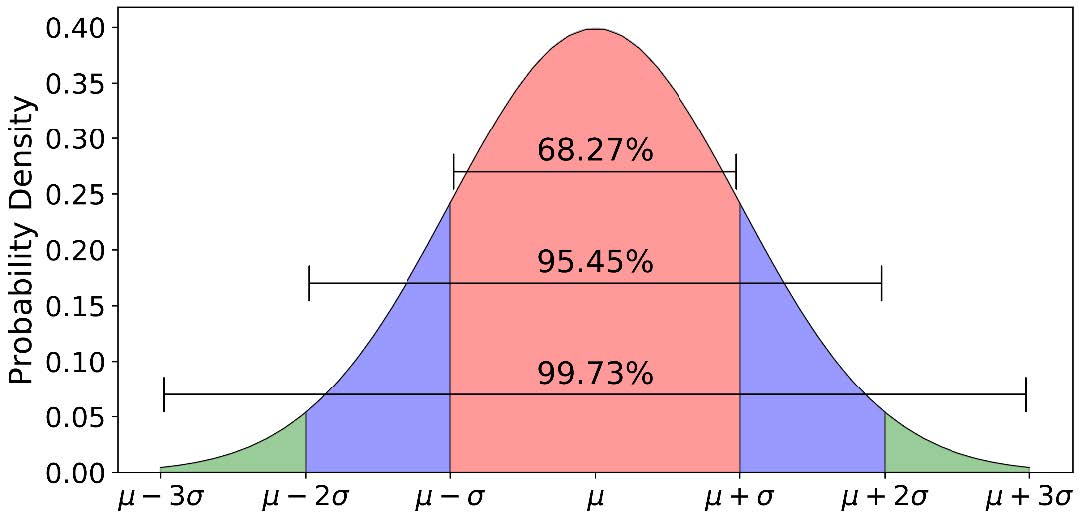
\includegraphics[width=\textwidth]{Images/Gaussiana.jpg}
    \caption{Gaussian probability distribution}
\end{figure}

Initial attempts to model P2P networks used random graph models, such as
the~\textbf{Erdös-Rényi} and \textbf{Watts-Strogatz} models. In these
models, links between nodes are formed with a certain probability,
resulting in a graph where the number of links per node follows a normal
(Gaussian) distribution (Figure 2.3). Most nodes have a similar number of
connections. However, research has shown that these random network
models~\textbf{seldom fit real-world P2P networks accurately}, as they
fail to capture the organizational patterns that emerge organically.

\subsubsection{Small-World Networks}

\begin{figure}[h]
    \centering
    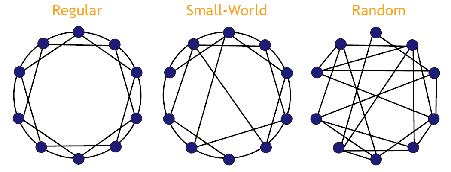
\includegraphics[width=\textwidth]{Images/Comparison of small world regular and random networks.jpg}
    \caption{Comparison of regular, small-world and random networks}
\end{figure}

A more accurate model for many real-world networks, including P2P
systems, is the~\textbf{Small-World Network}, also known as a power-law
or scale-free network. These networks are often described by
the~\textbf{Barabási-Albert model}, which is based on a principle
called~\textbf{"preferential attachment."}~This principle states that
new nodes joining the network are more likely to connect to existing
nodes that already have a high degree. In essence, popular nodes become
even more popular over time.

This leads to several key properties:

\begin{itemize}
\item
  \textbf{Hubs:}~The network contains a small number of highly connected
  nodes called~\textbf{hubs}, which have wide-ranging links to many
  other parts of the network. The vast majority of nodes have only a few
  local connections.
\item
  \textbf{Small Average Path Length:}~The hubs act as shortcuts,
  resulting in a surprisingly small average path length between any two
  nodes. This phenomenon is famously known as the "six degrees of
  separation" concept.
\end{itemize}

Clarifying examples of this are social networks. When we create a new
profile on a social network we are a node without links. One of the
first things we do is start following pages and the algorithm suggests
us to follow popular pages we could be interested in (preferential
attachment). When we are done creating our profile we are one of the
many modes with few links while the popular pages are few nodes with
many links (See figure 2.5).

\begin{figure}
      \centering
      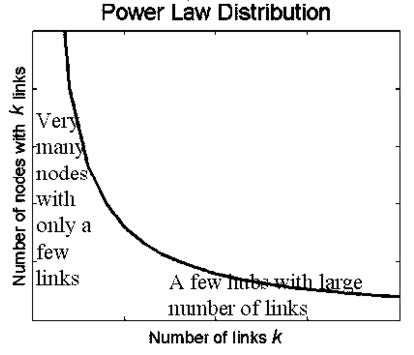
\includegraphics[width=\textwidth]{Images/Small world network power law.jpg}
      \caption{Power law distribution showing that there is a large number
      of nodes with few links and a small number of nodes with many links}
\end{figure}

To understand the "six degrees of separation" concept think about
LinkedIn. When we visit a profile of a person who is not in our network
we see a small number by their name: that is the number of intermediary
nodes between us and the other person. For instance, 2 means that there
are 2 people between us and the other person. The concept under
discussion states that given two random nodes they can be linked by
making a most of 6 hops in the network.

\subsubsection{Resilience Properties of Small-World Networks}

Small-world networks exhibit a fascinating duality in their resilience.
They are~\textbf{highly resilient to random node failures}. Because most
nodes have few links, the random removal of a node is unlikely to
disconnect the network. However, they are~\textbf{highly vulnerable to
targeted attacks against their hubs}. Removing just a few key hubs can
quickly partition the network into isolated, non-communicating segments.

Table 2.2 contains network experiments results that illustrate this contrast.

\begin{table}
    \centering
    \begin{tabularx}{\textwidth}{|X|X|X|} \hline
        \% of Random Node Failure & 10,000-Node Random Graph & 10,000-Node
        Power-Law Graph (Small-World) \\ \hline
        \textbf{5\%} & Largest component shrinks to 9,000 nodes. & Only a few
        isolated nodes break off. \\ \hline
        \textbf{18\%} & Only small components (1-100 nodes) remain. & Largest
        component is still \textasciitilde8,000 nodes. \\ \hline
        \textbf{45\%} & Only tiny groups (1-2 nodes) survive. & A large cluster
        persists alongside small fragments. \\ \hline
    \end{tabularx}
    \caption{Resilience comparison between random network graphs and small-world network graphs}
\end{table}

The data reveals a critical difference in how these network structures
degrade. In the random graph, the removal of 5\% of nodes (500 nodes)
causes an additional 500 nodes to become disconnected from the main
graph, a phenomenon known as network fragmentation. By contrast, the
power-law graph remains largely intact under the same failure rate due
to its reliance on hubs. This resilience against random failure comes at
a cost, as a targeted attack on those same hubs would cause catastrophic
failure.

In practice, these topologies are not implemented at the physical
network level but as~\textbf{overlay networks}, which are virtual
structures built on top of the physical Internet.

\chapter{P2P Overlay Networks}

\section{Introduction to P2P Overlay Networks}

Peer-to-Peer systems are not implemented directly on the physical
infrastructure of the internet. Instead, they are constructed as virtual
networks---known as~\textbf{overlay networks}---built on top of an
existing physical network. The topology of this overlay and the
strategies used for placing resources within it are fundamental design
choices that directly impact the system\textquotesingle s efficiency,
scalability, and overall functionality. This section classifies P2P
overlay networks based on these core architectural decisions.

\subsection{P2P Network Types}

\begin{figure}
  \centering
  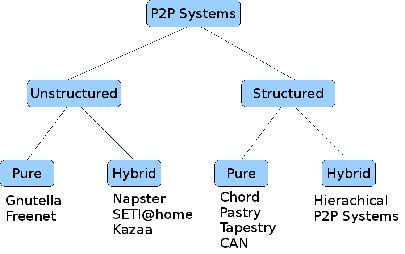
\includegraphics[width=0.8\textwidth]{Images/P2P overlay network types.jpg}
  \caption{P2P overlay network types}
\end{figure}

P2P overlay networks can be broadly divided into two main categories:
unstructured and structured (See figure 3.1).

\subsubsection{Unstructured P2P Networks}

This category describes networks in which there is no control over the
overlay topology or the placement of resources. Peers connect to each
other arbitrarily, and resources are stored on peers without a
coordinated plan. Consequently, locating a resource requires "blind"
search techniques that must propagate through the network.

\begin{itemize}
    \item
    \textbf{Pure Unstructured:}In this model, all nodes are equal,
    with no special roles or responsibilities. There is no control over how
    peers connect or where content is placed. This pure decentralization
    offers very high resilience to node failures but suffers from poor
    search efficiency and limited scalability, as queries can generate
    significant network traffic.
    
    \item 
    \textbf{Hybrid Unstructured:} This model introduces special nodes
    to improve efficiency. These nodes---variously known as~\emph{director
    nodes},~\emph{trackers}, or~\emph{super-peers}---assist with functions
    like peer lookup and content indexing. While this hybrid approach
    improves performance, these special nodes can become bottlenecks or
    single points of failure. Notable examples of hybrid systems
    include~\textbf{Napster},~\textbf{Skype}, and~\textbf{eDonkey}.
\end{itemize}

\subsubsection{Structured P2P Networks}

In contrast, structured networks employ decentralized self-organization
algorithms to exert precise control over both the network topology and
the placement of resources.

In this model, the system ensures that specific resources are placed at
specific, predictable locations, not on random peers. This organization
allows for highly efficient and targeted resource discovery.\\
The primary technology used to implement pure structured P2P networks is
the~\textbf{Distributed Hash Table (DHT)}.

Hybrid structured networks (e.g., multi-level, hierarchical) are
theoretically possible but they are rarely used in practice.

\subsection{Resource Discovery in Unstructured Networks}

In unstructured P2P networks, the lack of information about where a
specific piece of content is located necessitates the use of "blind"
resource discovery techniques. A peer initiating a search has no a
priori knowledge of which node holds the desired resource and must
therefore propagate its query across the overlay network. This section
analyzes the primary algorithms used for this purpose and evaluates
their operational complexity.

\subsection{Evaluating Blind Search Techniques}

The following are the most common blind search techniques, each with
distinct trade-offs between resilience and efficiency.

\subsubsection{Flooding}

\begin{table}
    \centering
    \begin{tabularx}{\textwidth}{|X|X|} \hline
            \adjustbox{max width=\linewidth}{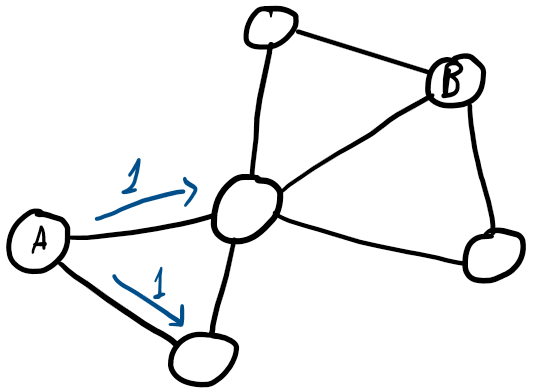
\includegraphics{Images/Flooding_1.png}}
            &
            \adjustbox{max width=\linewidth}{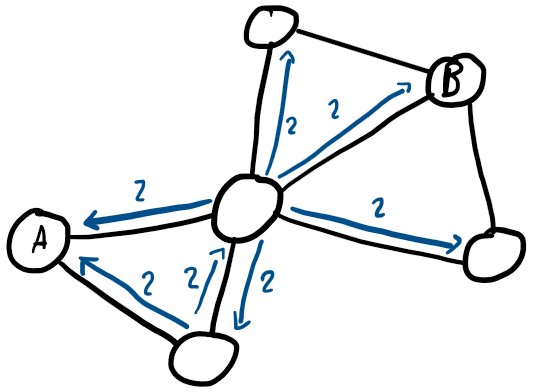
\includegraphics{Images/Flooding_2.png}} \\ \hline
            \adjustbox{max width=\linewidth}{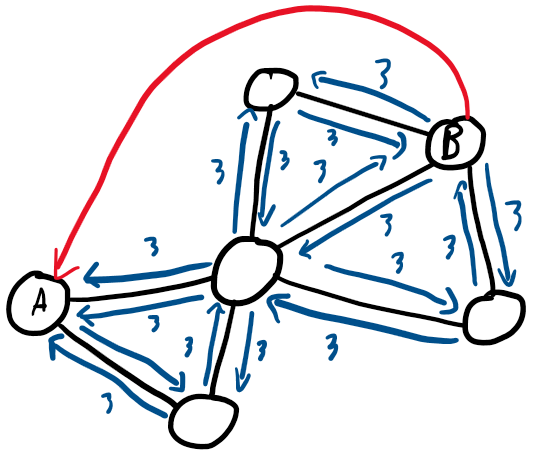
\includegraphics{Images/Flooding_3.png}}
            &
            \adjustbox{max width=\linewidth}{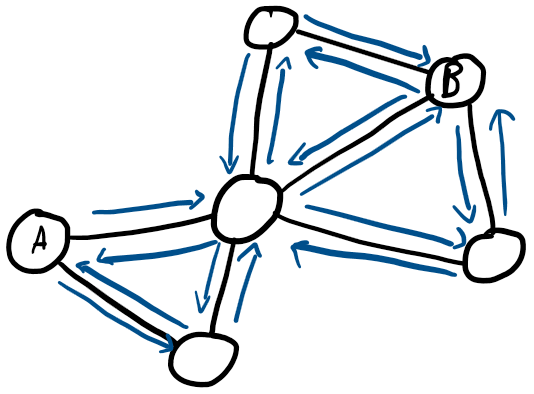
\includegraphics{Images/Flooding_4.png}} \\ \hline
    \end{tabularx}
    \caption{Flooding search example}
\end{table}

A requesting node sends a query message to all of its immediate
neighbors in the overlay network. Upon receiving the query, each
neighbor forwards it to~\emph{all}~of its neighbors. This process
repeats, causing the message to propagate throughout the entire
connected component of the network. Flooding offers maximum resilience,
as it is guaranteed to find an existing resource. However, it is highly
inefficient and scales poorly due to the massive duplication of
messages. Messages stop being forwarded in the network when the query
expires because the TTL (Time To Live) ends.

Now, let us analyze the figures in table 3.1. Let\textquotesingle s say that node A is
looking for a resource held by node B. In the first step, node A sends a
query to all its neighbors. In the second step, the central and bottom
nodes forward the query to all their neighbors and B receives the query.
In the third step B can communicate directly with A without forwarding
the resource to the intermediate nodes of the overlay network. Remember:
this is an overlay network and the nodes have access to the Internet.
Once two nodes know each other\textquotesingle s IP addresses they can
communicate directly through the Internet. The third picture also shows
the main inefficiency of the flooding algorithm. This algorithm is so
simple that it does not implement a strategy to stop forwarding useless
messages through the network so, even if the resource is found, nodes
will keep forwarding the query among one another until the TTL ends.
This means that the forwarding will continue even after the resource is
transferred to the requesting node as we can see in the fourth picture.

\subsubsection{Random Walk}

\begin{figure}
  \centering
  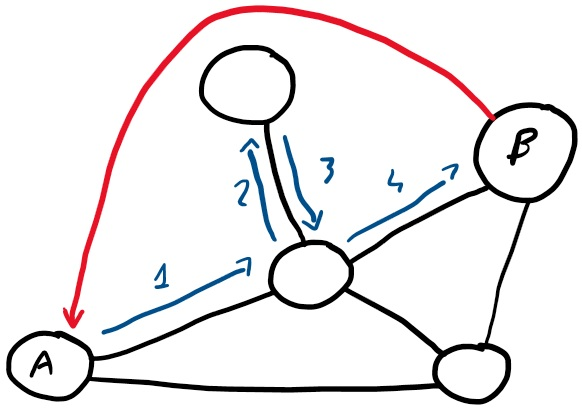
\includegraphics[width=0.8\textwidth]{Images/Random_walk.jpg}
  \caption{Random walk example}
\end{figure}

A requesting node forwards a query to a single, randomly selected
neighbor. That neighbor, in turn, forwards it to one of its own randomly
selected neighbors. This process continues for a predetermined number of
steps (TTL). This technique is simple to implement and generates very
little network traffic, but it does not guarantee complete network
coverage and may fail to find an existing resource.

\subsubsection{Expanding Ring}

\begin{figure}
  \centering
  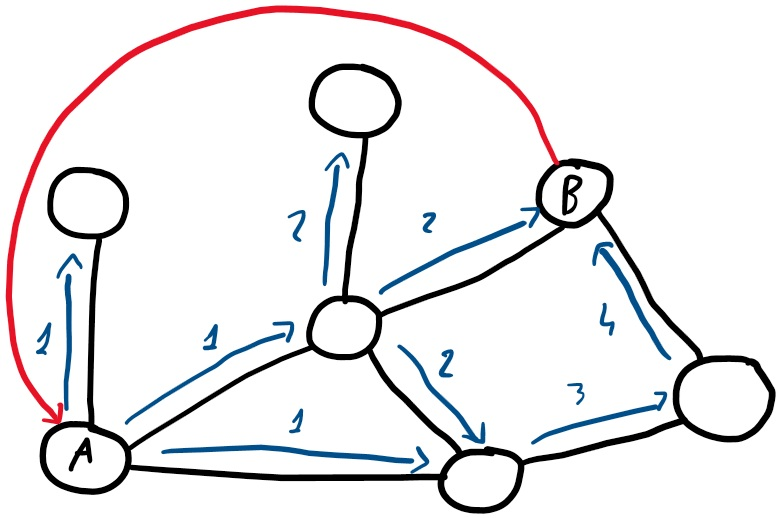
\includegraphics[width=0.8\textwidth]{Images/Expanding_ring.jpg}
  \caption{Expanding ring example}
\end{figure}

This technique is a controlled variation of flooding. Each query message
is issued with a limited "time-to-live" (TTL), typically measured as a
hop count. When a node forwards the query, it decrements the TTL. A node
that receives a message with a TTL of zero will process the request but
will not forward it further. This constrains the search to a specific
radius within the network, limiting the message overhead at the cost of
potentially incomplete coverage.

This algorithm implements what we ideally expect from the flooding
search because nodes do not forward messages to the node from which they
received it so the query can only go forward.

\subsubsection{Analyzing the Time Complexity of Flooding Search}

The communication overhead, or time complexity, of a flooding search is
a critical factor limiting its scalability. In a densely connected
network with $N$ nodes, the complexity is $\geq O(N^2)$.

This quadratic complexity arises because the search generates an
explosive amount of message traffic. In a densely connected network,
each of the $N$ nodes can receive the query and forward it to its
approximately $N-1$ other neighbors. This leads to a number of messages
proportional to the square of the number of nodes, making the flooding
approach unsustainable for large-scale P2P systems. The quadratic
communication overhead of flooding makes it fundamentally unscalable for
large networks, creating a critical need for an alternative approach
that could provide efficient, targeted discovery without sacrificing
decentralization. This need is directly addressed by structured networks
and their use of Distributed Hash Tables.

\subsection{Resource Discovery in Structured Networks: Distributed
Hash Tables
(DHTs)}\label{resource-discovery-in-structured-networks-distributed-hash-tables-dhts}

Structured P2P networks solve the resource discovery problem by imposing
a specific, predictable organization on both the network topology and
its data. The fundamental technology that enables this organization is
the~\textbf{Distributed Hash Table (DHT)}. DHTs provide a scalable and
efficient lookup service that allows peers to locate resources with a
precision and speed unattainable in unstructured networks.

\subsubsection{Explaining the Fundamentals of
DHTs}

\begin{figure}
  \centering
  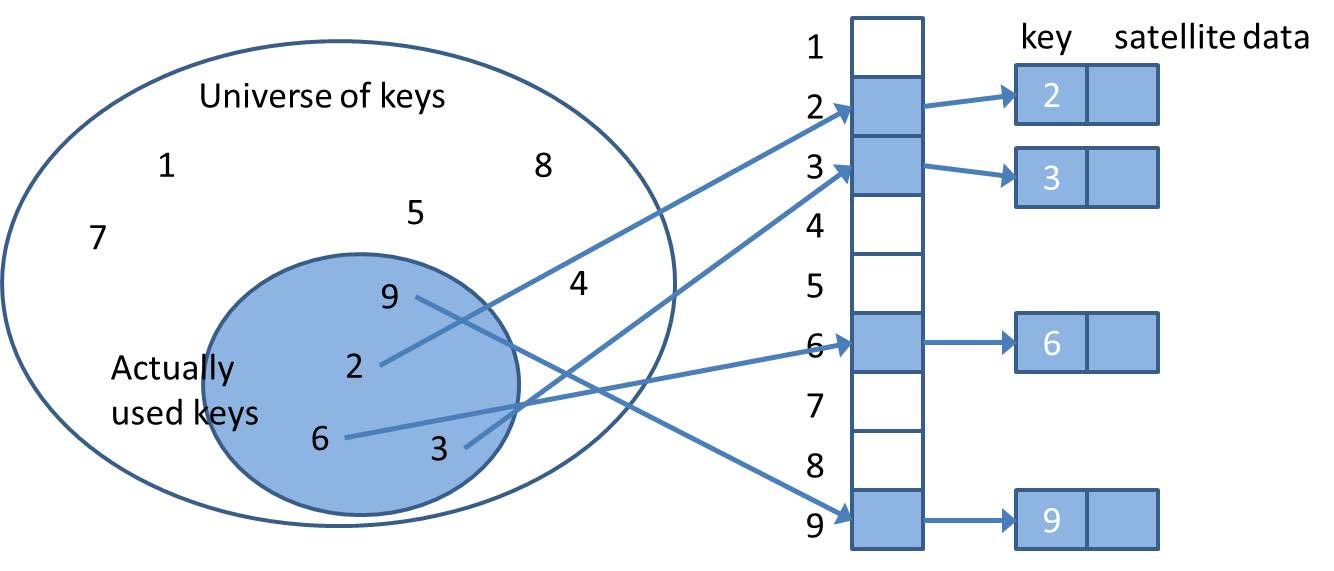
\includegraphics[width=0.8\textwidth]{Images/Hash table.jpg}
  \caption{Hash table}
\end{figure}

A standard \textbf{hash table} is a data structure that maps keys to values.
It consists of an array of slots, or \textbf{buckets}, and a \textbf{hash
function} that computes a bucket index for any given key. This allows
for constant-time $(O(1))$ insertion, deletion, and lookup operations.

\begin{figure}
  \centering
  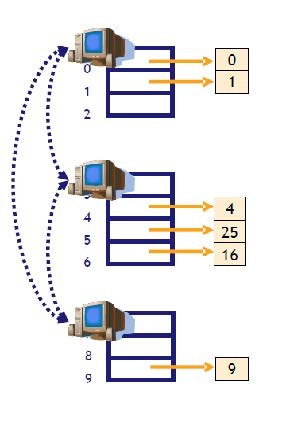
\includegraphics[width=0.8\textwidth]{Images/Distributed hash table.jpg}
  \caption{Distributed hash table}
\end{figure}

The core idea of a DHT is to distribute this hash table across all the
peers in the network. The array of buckets is partitioned, and each peer
becomes responsible for managing a specific portion of the key space.
When a peer wants to store or retrieve a resource, it first calculates
the resource\textquotesingle s key using a shared hash function. The DHT
protocol then routes the request to the peer responsible for that key.
To handle "churn" (nodes joining and leaving), DHTs typically employ
redundancy, ensuring that resources managed by a departing node are not
lost.

\subsubsection{Clarifying the DHT Routing Process}

\begin{figure}
  \centering
  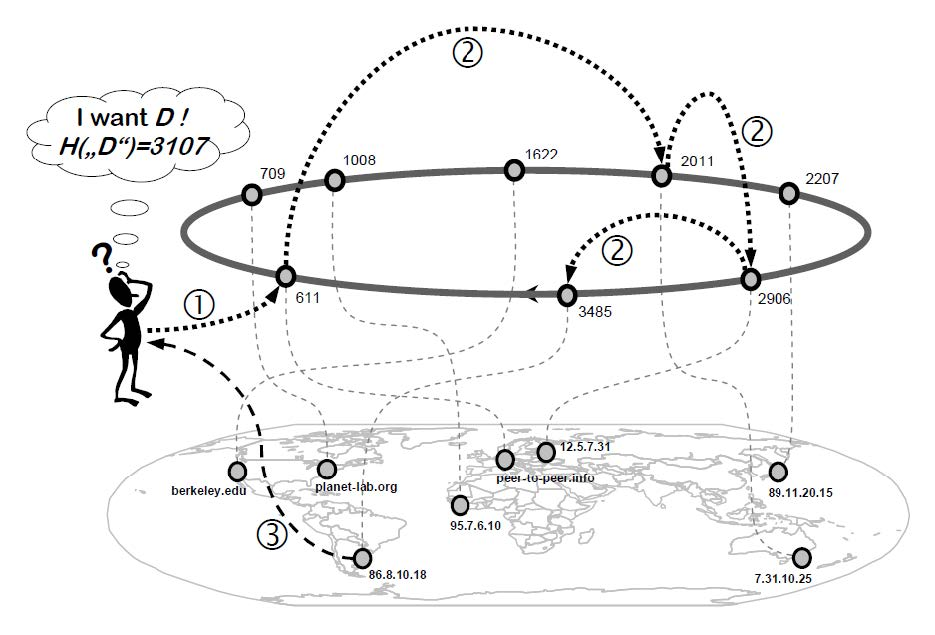
\includegraphics[width=0.8\textwidth]{Images/DHT routing.jpg}
  \caption{DHT routing process}
\end{figure}

A critical question in a DHT is how a peer can find the specific node
responsible for a given key when it does not possess a map of the entire
network. The process is accomplished through a collaborative, iterative
routing algorithm.

\begin{enumerate}
    \item
    \textbf{Key Computation:} A peer wishing to retrieve a resource first computes the resource\textquotesingle s key by applying a globally
    known, shared hash function (e.g., SHA-1) to an identifier for that
    resource.

    \item 
    \textbf{Request Initiation:} The requesting peer does not know which node is responsible for that key. It initiates the process by sending its lookup request to an \emph{arbitrary} or \emph{neighboring} peer
    that it already knows about.

    \item 
    \textbf{Iterative Forwarding:} Each peer in a DHT maintains a local routing table containing information about a small subset of other peers. When a peer receives a lookup request, it uses this local information to forward the request to another peer that is "closer" to the target key according to a predefined distance metric.
    
    This process is analogous to addressing a letter to a recipient in a foreign country. One does not need to know the recipient\textquotesingle s exact street address to begin; you simply
    route it to the correct country. The national postal service then routes
    it to the correct state or province, which routes it to the city, and
    finally to the local post office---each step leverages local knowledge
    to bring the message progressively closer to its final destination.

    \item 
    \textbf{Convergence:}~This iterative process continues, with each hop bringing the request progressively closer to its destination. The
    request eventually reaches the peer responsible for the target key. This
    process is highly efficient, typically completing in $O(log N)$ hops for a network with N nodes.
\end{enumerate}

Once the responsible peer is located, it can communicate directly with
the original requester to transfer the resource.

\subsubsection{Why does a requesting node contact an arbitrary DHT node instead of hashing and contacting the owner directly?}

This question addresses a core principle of decentralized systems: the
avoidance of global state. In a scalable DHT, it is a design axiom that
no single node can or should possess a complete map of the network. A
node initiates a search by contacting any node it~\emph{does}~know, such
as a neighbor or a pre-configured bootstrap node. This entry-point node
then uses its local routing information (its finger table) to forward
the request to another node that is~\emph{provably closer}~to the target
key\textquotesingle s successor. This multi-hop process is repeated,
with each hop getting progressively closer, until the target node is
found. Peers do not know the buckets of all other nodes, as maintaining
such a global state would defeat the purpose of a decentralized,
scalable system.

\subsubsection{What are the numbers on the ring and how do nodes communicate?}

The numbers on the ring are the~\textbf{Node IDs}, which are assigned
from the same identifier space as the resource keys. Communication
is~\textbf{not random}. When a node needs to forward a request for a
key~\texttt{k}, it consults its finger table and identifies the known
node whose ID most closely precedes~\texttt{k}. It then forwards the
request to that node. This makes the largest possible "jump" toward the
destination in a deterministic and efficient manner.

\section{Case Studies in DHT Implementation}

While the core principles of a Distributed Hash Table are
consistent---mapping keys to responsible nodes---different systems
implement the overlay topology and routing logic in unique ways. These
design choices result in different performance characteristics and
trade-offs. This section will explore three seminal and influential DHT
implementations:~\textbf{Chord},~\textbf{CAN}, and~\textbf{Kademlia}.

\subsection{Analyze Chord\textquotesingle s Ring Topology}

\begin{table}
    \centering
    \begin{tabularx}{\textwidth}{|X|X|} \hline
            \adjustbox{max width=\linewidth}{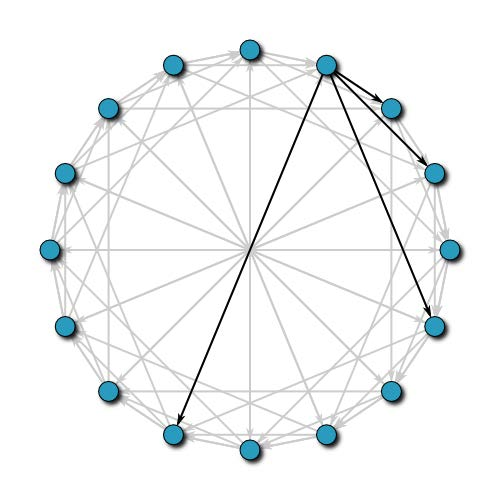
\includegraphics{Images/Chord routing without finger table.jpg}}
            &
            \adjustbox{max width=\linewidth}{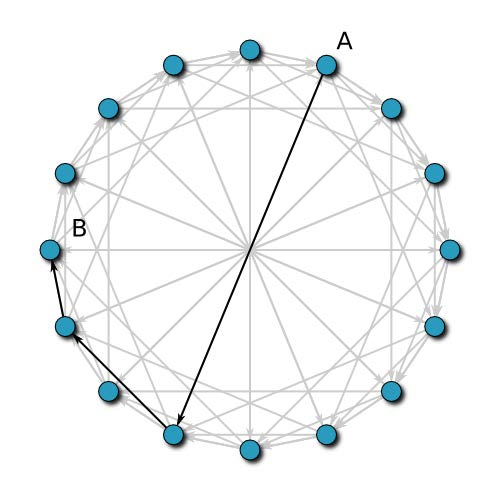
\includegraphics{Images/Chord routing with finger table.jpg}} \\ \hline
    \end{tabularx}
    \caption{Chord routing without finger table (on the left) and with finger table (on the right)}
\end{table}

Chord organizes its peers into a logical \textbf{ring}. Each peer is assigned
a numerical ID, and its position on the ring is determined by this ID.

\begin{itemize}
\item
  \textbf{Resource Mapping:}~A resource with a key~\texttt{k}~is managed
  by the peer whose ID is the first to succeed~\texttt{k}~on the ring.
  This peer is known as the~\texttt{successor}~of~\texttt{k}. Formally,
  the responsible node is the one with the smallest ID that is greater
  than or equal to~\texttt{k}.
\item
  \textbf{The Finger Table:}~If a peer only knew its immediate
  successor, a search for a key on the other side of the ring would
  require traversing half the network---a linear search with $O(N)$
  complexity. To solve this, each peer maintains a~\textbf{finger
  table}. This table acts as a list of shortcuts, storing the addresses
  of other peers at geometrically increasing distances around the ring
  (e.g., the peer at distance 1, 2, 4, 8, etc.). When routing a request,
  a peer can use its finger table to jump to a node that is much closer
  to the target key, bypassing many intermediate nodes. This mechanism
  dramatically reduces the search complexity to logarithmic
  time, $O(log N)$.
\end{itemize}

\subsection{Analyze CAN\textquotesingle s Coordinate Space Topology}

The Content-Addressable Network (CAN) implements its DHT using a
virtual~\textbf{d-dimensional Cartesian coordinate space}. This logical
space is completely independent of the physical network.

\begin{itemize}
\item
  \textbf{Resource Mapping:}~The entire coordinate space is dynamically
  partitioned among all nodes, with each node "owning" a distinct zone.
  A resource\textquotesingle s key is mapped to a point in this space
  using~\texttt{d} separate hash functions---one for each dimension. The
  node whose zone contains this point is responsible for storing and
  managing the resource.
\item
  \textbf{Greedy Routing:}~Routing is performed greedily based on
  Cartesian distance. When a node receives a request for a key, it
  forwards the request to the neighbor whose zone is closest to the
  destination coordinates. This iterative process continues until the
  request reaches the node that owns the target zone. The time
  complexity for a search in an N-node network
  with~\texttt{d}~dimensions is {}.
\item
  \textbf{Node Joining}: When a new node joins, it first discovers an
  existing node to get an entry point into the network. It then picks a
  random point in the coordinate space and sends a join request,
  directed to that point, through the network. The node currently owning
  the zone containing that point receives the request and splits its
  zone in half, retaining one half and assigning the other half to the
  new node.
\item
  \textbf{Node Leaving}: When a node leaves the network, its formerly
  assigned zone is distributed to its neighbors through a merging or
  takeover process. Merging is preferred over takeover because the
  merging process has a preliminary check phase in which nodes make sure
  that the potentially merged area is geometrically valid which, in this
  case, means that the resulting region is simply connected. Ideally, we
  want region to be simply connected because we want to avoid what would
  happen otherwise. If a region wasn\textquotesingle t simply connected
  it would mean that while traversing the network between two points
  belonging to the same node we would pass through a region of another
  node as shown in figure 3.7.

\begin{figure}
  \centering
  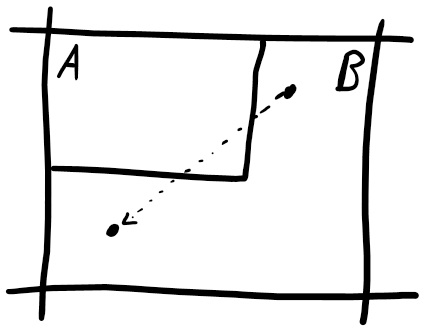
\includegraphics[width=0.8\textwidth]{Images/CAN not simply connected region.jpg}
  \caption{CAN routing through another region}
\end{figure}

  In conclusion, when a node leaves the network its neighbors perform
  the following steps:
  
  \begin{enumerate}
  
  \item 
  \textbf{Merge feasibility check:} The neighbors
  check if the abandoned area can be merged to the area of another node
  to create a simply connected area.
  
  \item 
  \textbf{Merging:} If merging the
  areas is feasible they are merged and the neighbors update their
  routing tables to consider the change in the topology of the network.

  \item
  \textbf{Takeover:} If merging the areas is infeasible the neighbor of
  the abandoned area whose controlled region is smallest takes control
  of the abandoned area. After the takeover, the new owner of the area
  can periodically try to merge its region with the ones of the
  neighbors to form a simply connected region.
  
  \end{enumerate}
\end{itemize}

\subsubsection{How do the nodes know if a node leaves the
network?}

CAN networks are designed to be scalable, fault tolerant and
self-organizing. A node can leave the network either voluntarily or
because of a fault so, CAN networks have to consider both cases. \\ \\
In a CAN network nodes communicate periodically with their neighbors
sending \textbf{heartbeat messages} which are periodic messages meant to
signal their presence in the network. By the time a neighboring node
does not receive an heartbeat message from a node for a given period of
time, it understands that the node left the network. This happens
regardless of the node leaving the network voluntarily or not so this is
how nodes understand if a node left the network because of a fault. \\ \\
In case a node voluntarily leaves the network it sends a specific
message to their neighbors to signal its exit.

\subsubsection{Clarifying examples}

\begin{figure}
  \centering
  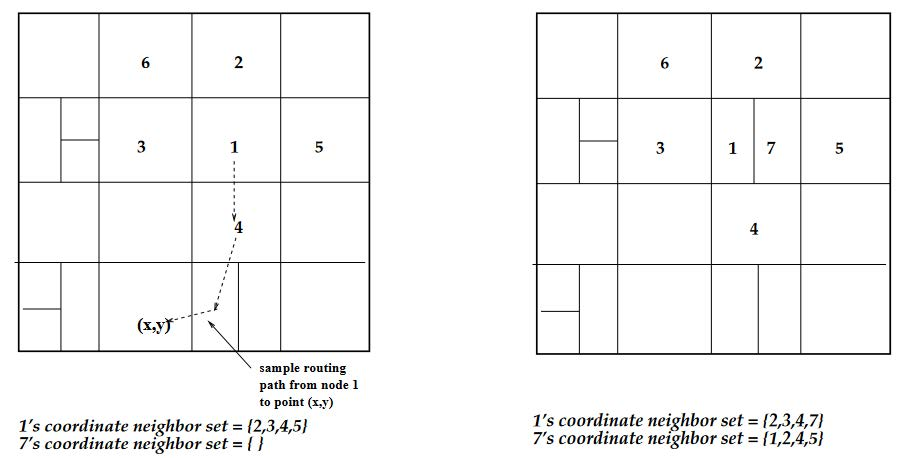
\includegraphics[width=0.8\textwidth]{Images/CAN routing.jpg}
  \caption{CAN routing example (on the left) and node joining the network (on the right)}
\end{figure}

In the left part of figure 3.8 we can see an example of routing from
node 1 to the point $(x,y)$. Before we start covering the greedy
routing process we need to make an important premise: all areas in the
picture are managed by a node even if there isn\textquotesingle t an
identifier.

To understand greedy routing think about the greedy search (Informed
search algorithm covered during the Agent Based Artificial Intelligence
course). In the greedy search we perform the most advantageous move in
each step considering only the initial situation of each step. We
don\textquotesingle t ask ourselves if it is the best move possible
considering the whole path as we do in A* search.

Greedy routing follows the same philosophy: given the current position,
which neighbor has a coordinate which is closest to the ones of the
point I want to reach?

In the picture we have that both the $x$ and $y$ coordinates of the target
point are smaller than the ones of the starting node 1. This means that
the next move can either be to the left or downwards. In this example
node 1 contacts node 4 because it arbitrarily decided to minimize the $y$
coordinate gap first. Node 4 has two neighbors below it which have the
same $y$ coordinate but different $x$ coordinates. In this case the best
step of the greedy routing process consists in choosing the bottom left
neighbor. Now the last step consists in contacting the neighbor on the
left.

If, instead, node 1 decided to minimize the $x$ coordinate gap first it
would have contacted node 3 and henceforth the query would have been
forwarded downwards until reaching the target point.

Greedy algorithms are a recurring topic in P2P networks because there
doesn\textquotesingle t exist a global state. So, even if we wanted to
implement an optimal strategy using the same philosophy as the A*
search, we couldn\textquotesingle t do that because nobody knows the
whole network.

On the right part of figure 3.8 we see node 7 joining the network. When
node 7 joined the network it randomly picked a position in the area
managed by node 1 so the area formerly managed by node 1 is now split
into two parts.

\subsection{Analyze Kademlia\textquotesingle s Binary Tree Topology}

\begin{figure}
  \centering
  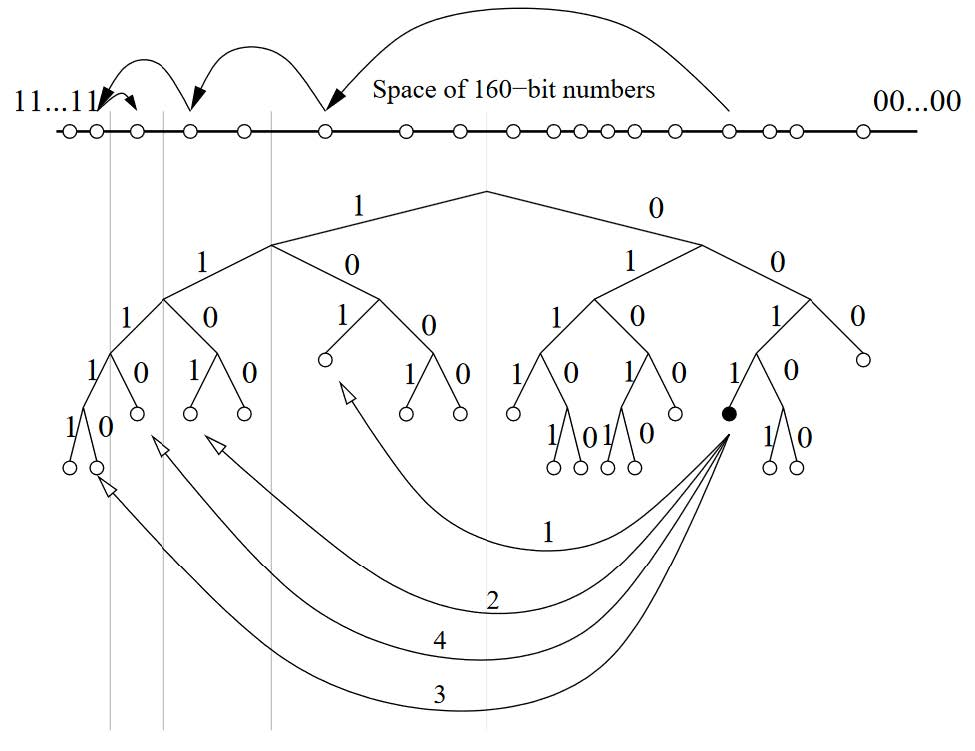
\includegraphics[width=0.8\textwidth]{Images/Kademlia.jpg}
  \caption{Kademlia's binary tree}
\end{figure}

Kademlia structures its overlay network as a \textbf{binary tree}. Each node
is assigned a random N-bit ID (e.g., 160 bits), which determines its
position as a leaf in the tree.

\begin{itemize}
\item
  \textbf{XOR-Based Distance Metric:} Unlike Chord\textquotesingle s
  linear distance on a ring, Kademlia defines the distance between two
  node IDs as the numerical result of their~\textbf{Bitwise Exclusive OR
  (XOR)}. This metric has the useful property that it is symmetric and
  allows the network to be partitioned systematically.
\item
  \textbf{The k-bucket Mechanism:}~To manage its routing information,
  each Kademlia node maintains a set of lists called~\texttt{k-buckets}.
\end{itemize}

A \texttt{k-bucket} is a list containing up to \texttt{k} entries (where \texttt{k} is a system parameter, like 20). Each entry stores the
IP address, port, and ID of another known node. \\ \\
A node maintains a separate \texttt{k-bucket} for different ranges of XOR distance from itself. These ranges are defined by the position of
the most significant bit in which a remote node\textquotesingle s ID differs from its own. For an N-bit ID space, there are N \texttt{k-buckets}. This structure ensures a node maintains a rich, detailed list of many "close" neighbors (where the first differing bit is far to the right) and progressively sparser lists of nodes that are farther away.

\subsubsection{k-buckets examples}
Consider a node with an ID starting with
  \texttt{10110...}. This node maintains separate k-buckets to keep
  contacts in different sub-trees of the network.
  \begin{itemize}
      \item
      One bucket stores up to \texttt{k} nodes whose IDs start
      with \texttt{0...} (differing at the 1st bit).

      \item
      Another bucket stores up to \texttt{k} nodes whose IDs start with \texttt{11...} (sharing the first bit, but differing at the
      2nd).

      \item
      A third bucket stores nodes starting with \texttt{100...} (sharing
      the first two bits, differing at the 3rd), and so on.
  \end{itemize}

\subsubsection{Why this structure is effective} This clever partitioning allows a node to quickly find a contact in the specific sub-tree where
  a target key must reside. This bitwise partitioning is what gives the
  XOR metric its power; the \textquotesingle distance\textquotesingle{}
  calculated by XOR(\texttt{ID1},~\texttt{ID2}) directly corresponds to
  the first bit where the nodes diverge, placing them in a predictable
  sub-tree and k-bucket relative to one another. By forwarding a request
  to a node in the appropriate k-bucket, the routing algorithm
  effectively halves the remaining "distance" to the target with each
  hop. This guarantees logarithmic $O(log N)$ performance.

\subsubsection{Illustrating Kademlia Routing} Kademlia\textquotesingle s
  routing is a~\textbf{greedy routing}~algorithm. At each step, a node
  forwards a request to the node in its~\texttt{k-buckets}~that is
  closest to the final destination according to the XOR distance metric.
  Consider an example where node~\texttt{0011}~wants to find
  node~\texttt{1110}:

\begin{enumerate}
    \item
    \textbf{Start:} Node \texttt{0011} calculates its XOR distance to the target \texttt{1110}: \texttt{d(0011,\ 1110)\ =\ 0011\ XOR\ 1110\ =\ 1101}.

    \item 
    \textbf{Hop 1:} Node \texttt{0011} consults
    its \texttt{k-buckets} to find the known node that minimizes the XOR distance to \texttt{1110}. Let\textquotesingle s assume this node
    is \texttt{0101}. It forwards the request to \texttt{0101}. The new
    distance is \texttt{d(0101,\ 1110)\ =\ 0101\ XOR\ 1110\ =\ 1011}.
    Since \texttt{1011} is smaller than the previous distance \texttt{1101}, the search is getting closer.
    
    \item
    \textbf{Hop 2:} Node \texttt{0101} repeats the process, consulting its own \texttt{k-buckets}. It finds that~\texttt{1101}~is
    its closest known peer to the target. It forwards the request there. The
    new distance is~\texttt{d(1101,\ 1110)\ =\ 1101\ XOR\ 1110\ =\ 0011}.
    The distance has shrunk significantly.

    \item \textbf{Convergence:} Node \texttt{1101} would then consult its \texttt{k-buckets} and find the final destination, \texttt{1110}.
    Each step in this path represents a greedy choice that brings the query
    closer to the target, ensuring the search converges quickly with a time
    complexity of $O(log N)$.
\end{enumerate}

\subsection{Comparative Analysis of P2P Architectures}

The choice of a particular P2P architecture---or choosing between P2P
and a centralized model---involves significant trade-offs between
implementation complexity, operational efficiency, and system
robustness. This final section provides a systematic comparison of the
main architectural approaches discussed, evaluating them against a set
of key metrics that capture these trade-offs.

\subsection{Defining the Evaluation Metrics}

To compare different distributed system architectures, we can use the
following metrics:

\begin{itemize}
\item
  \textbf{Per Node State:}~This metric, also known as space complexity,
  refers to the amount of routing information or other state that each
  individual node must maintain about the rest of the network. A lower
  per-node state is generally preferable for scalability.
\item
  \textbf{Communication Overhead:}~This metric, also known as time
  complexity, measures the number of messages required to perform a
  standard operation, such as a resource lookup. Lower overhead
  indicates greater efficiency.
\item
  \textbf{Complex Query Patterns:}~This refers to the
  system\textquotesingle s ability to support searches that are not
  based on an exact, known key. Examples include keyword searches,
  multi-parameter queries, or range queries.
\item
  \textbf{Robustness:}~This defines the system\textquotesingle s ability
  to continue functioning correctly despite nodes frequently joining,
  leaving (an event known as churn), or failing unexpectedly.
\end{itemize}

\subsection{Presenting and Analyzing the Comparison Table}

\begin{figure}
  \centering
  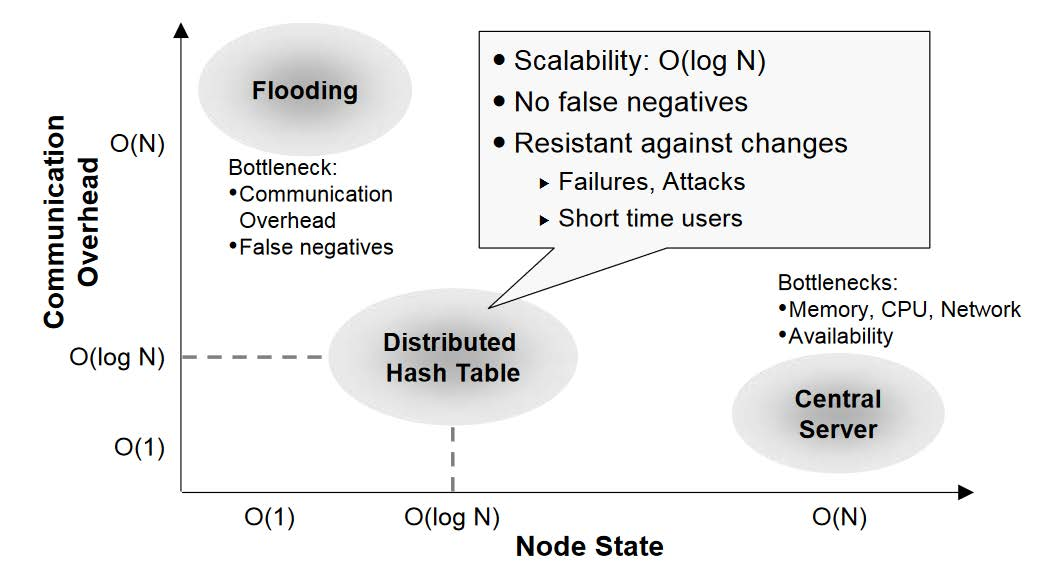
\includegraphics[width=0.8\textwidth]{Images/Distributed architecture comparison.jpg}
  \caption{Distributed architecture comparison}
\end{figure}

Table 3.3 summarizes the performance of three primary architectures against these metrics.

\begin{table}
    \centering
    \begin{tabularx}{\textwidth}{|X|X|X|X|X|} \hline
        System & Per Node State & Communication Overhead & Complex Query
        Patterns & Robustness \\ \hline
        \textbf{Central server} & $O(N)$ & $O(1)$ & Yes & No \\ \hline
        \textbf{Flooding search} & $O(1)$ & $\geq O(N^2)$ & Yes & Yes \\ \hline
        \textbf{DHT} & $O(log N)$ & $O(log N)$ & No & Yes \\ \hline
    \end{tabularx}
    \caption{Architecture performance comparison}
\end{table}

A detailed analysis of each model reveals their inherent trade-offs:

\begin{itemize}
\item
  \textbf{Central Server:}~This architecture provides excellent
  performance for lookups, as a client can query the server directly in
  constant time ($O(1)$). The server can also easily support
  complex queries. However, this comes at the cost of scalability and
  robustness. The server must maintain state for all $N$ nodes in the system ($O(N)$), and its failure will bring down the entire
  network, making it \textbf{not robust}.
\item
  \textbf{Flooding Search (Unstructured P2P):}~This model offers maximum
  robustness, as the failure of any single node has little impact on the
  overall network. Each node also has a minimal state requirement,
  needing only to know its immediate neighbors ($O(1)$). However,
  its communication overhead is quadratic ($\geq O(N^2)$), making it
  highly inefficient and unscalable. It does, however, naturally support
  complex queries, as a query can contain any pattern to be matched by
  receiving peers.
\item
  \textbf{DHT (Structured P2P):} This model represents a highly
  effective compromise. It achieves an excellent balance where both the
  per-node state and the communication overhead are logarithmic ($O(log N)$).
  This makes DHTs highly scalable. Like flooding-based systems, DHTs are \textbf{robust} due to their decentralized nature and built-in
  redundancy mechanisms. Their primary limitation is that basic DHTs do not support complex query patterns, as lookups are tied to exact keys
  computed via a hash function. However, it is worth noting that more sophisticated DHT approaches have been proposed in academic literature to address this limitation.
\end{itemize}

\chapter{Foundational Concepts for Trustworthy Systems}

\begin{figure}
  \centering
  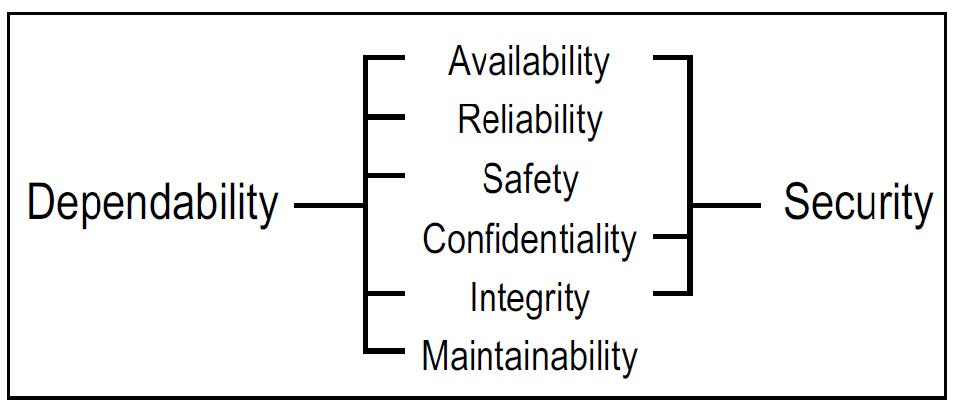
\includegraphics[width=0.8\textwidth]{Images/Distributed system properties.jpg}
  \caption{Trustworthy system properties}
\end{figure}

Before delving into the specific mechanisms of transactional systems, it
is crucial to establish the broader properties that define a trustworthy
computational system. These foundational pillars of security and
reliability are precisely what transactions are designed to protect and
uphold. A system that can be trusted is one that is dependable,
resilient, and secure.

The three core pillars of a trusted system are:

\begin{itemize}
\item
  \textbf{Dependability:}~This property signifies that users can rely on
  the system to function and operate correctly. It encompasses several
  key attributes:

  \begin{itemize}
  \item
    \texttt{availability}: The readiness of the system for correct
    service.
  \item
    \texttt{reliability}: The continuity of correct service over time.
  \item
    \texttt{safety}: The absence of catastrophic consequences for users,
    information, and the surrounding environment.
  \item
    \texttt{integrity}: The prevention of improper system alterations.
    This includes both \emph{data integrity}, which ensures that
    information managed by the system is not tampered with, and \emph{system integrity}, which prevents the configuration and
    behavior of system nodes from being controlled by an unauthorized entity.
  \item
    \texttt{maintainability}: The ability of the system to undergo necessary modifications and repairs.
  \end{itemize}
\item
  \textbf{Resilience:} Resilience is fundamentally achieved
  through~\texttt{fault\ tolerance}, which is the ability of a system to
  avoid service failures even in the presence of faults affecting its
  components, such as individual nodes or communication links. Fault
  tolerance is the primary mechanism by which a system achieves the
  property of reliability.


\item 
    \textbf{Security:} While security incorporates the properties of \texttt{availability} and \texttt{integrity} from dependability, it adds a critical third dimension: \texttt{confidentiality}, which is the prevention of unauthorized disclosure of information.
\end{itemize}

These high-level system goals are achieved through specific
architectural models and protocols. The transactional model provides a
powerful framework for implementing these guarantees in data-centric
applications.

\section{Foundational Concepts of Transactional Systems}

A transactional system is a fundamental paradigm for reliable
information processing, allowing for complex operations to be executed
with guarantees of correctness and stability. This section establishes
the core definition and lifecycle of a transaction, which serves as the
basic unit of work in such systems. By understanding its structure and
potential outcomes, we can build a foundation for exploring the
properties that make these systems robust.

A \textbf{transaction} is defined as a sequence of operations on resources. Its structure is formally encapsulated between
a \texttt{Begin\ of\ Transaction\ (bot)} operation, which marks its start, and an \texttt{End\ of\ Transaction\ (eot)} operation, which marks its conclusion.

A well-formed transaction has two possible outcomes, determined by a
specific command executed immediately before the \texttt{eot} marker:

\begin{enumerate}
    \item 
    \textbf{Commit work (commit):}~This signifies that all operations within the transaction have succeeded and their effects should be made permanent.

    \item 
    \textbf{Roll back (abort):} This signifies that the transaction has failed for some reason and all its partial effects must be undone, leaving the system in the state it was in before the transaction began.
\end{enumerate}

Crucially, once a \texttt{commit} or \texttt{abort} command is executed,
no further operations on resources can occur within that transaction. The transaction model is versatile and can encompass several types of
actions, including:

\begin{itemize}
\item
  Changes to stored data
\item
  Communications with external entities (e.g., sending a message)
\item 
Actions on transducers (e.g., sensors or actuators)
\end{itemize}

To be considered reliable, every transaction must strictly adhere to a
specific set of properties. These guarantees, collectively known as
ACID, are the cornerstone of transactional integrity.

\section{The ACID Properties: Guarantees of Transactional Integrity}

The strategic importance of the ACID properties cannot be overstated;
they are a set of four guarantees that ensure data validity and
reliability in database systems, even in the event of errors, power
failures, or other disruptions. The term~\textbf{ACID}~is an acronym for
Atomicity, Consistency, Isolation, and Durability, coined by Andreas
Reuter and Theo Härder in 1983 to formalize the principles of
transaction-oriented processing.

\subsection{Atomicity}

Atomicity guarantees that each transaction is treated as a single,
indivisible "unit" of work, which either succeeds completely or fails
completely. If any statement or operation within the transaction fails,
the entire transaction is rolled back, and the database is left
unchanged. This "all-or-nothing" principle prevents partial updates that
could corrupt the system\textquotesingle s state.

\textbf{Example:}~A monetary transfer from one bank account to another
consists of two operations: debiting the source account and crediting
the destination account. Atomicity ensures that if the credit operation
fails for any reason, the debit operation is also undone. The money is
neither lost nor created, preserving the integrity of the accounts.

\subsection{Consistency}

Consistency ensures that a transaction can only transition the database
from one valid state to another, preserving all predefined rules and
invariants. Any data written to the database must be valid according to
all constraints, cascades, and triggers. This property prevents illegal
transactions from corrupting the data.

\textbf{Example:}~Consider a database with an integrity constraint that
for two columns,~\texttt{A}~and~\texttt{B}, the
sum~\texttt{A\ +\ B}~must always equal 100. A transaction that
successfully subtracts 10 from~\texttt{A}~but fails to
alter~\texttt{B}~would violate this rule (\texttt{A\ +\ B}~would equal
90). The consistency guarantee ensures this transaction would be
aborted, and the database would be rolled back to its previous
consistent state where~\texttt{A\ +\ B\ =\ 100}.

\subsection{Isolation}

Isolation ensures that the concurrent execution of transactions leaves
the database in the same state that would have been obtained if the
transactions were executed sequentially. In other words, the operations
of one transaction are not visible to other concurrent transactions
until it is complete. This prevents interference between transactions
that are active in overlapping time frames.

\textbf{Example:}~To demonstrate a failure of isolation, consider two
transactions:~\texttt{T1}~transfers 10 from account A to B,
and~\texttt{T2}~transfers 20 from B to A. If their operations were
interleaved improperly, the sequence might be:

\begin{enumerate}
    \item
    \texttt{T1} subtracts 10 from A.

    \item
    \texttt{T2} subtracts 20 from B.

    \item
    \texttt{T2} adds 20 to A.

    \item
    \texttt{T1} adds 10 to B.
\end{enumerate}

If~\texttt{T1}~were to fail at this point, its effects would be rolled
back. However,~\texttt{T2}~has already modified account A and committed.
Reverting~\texttt{T1}~would mean adding 10 back to A, but this would
erase~\texttt{T2}\textquotesingle s modification, leaving the database
in an invalid state. This is a "write-write contention." Isolation
prevents such scenarios by ensuring that from each
transaction\textquotesingle s perspective, other transactions have
either already completed or not yet begun.

\subsection{Durability}

Durability guarantees that once a transaction has been successfully
committed, its effects will persist indefinitely, even in the event of a
system failure like a power outage or crash. This is typically achieved
by recording the completed transaction\textquotesingle s effects in
non-volatile memory.

\textbf{Example:}~After a user receives confirmation that a fund
transfer was successful, durability ensures that the change is
permanently recorded. Even if the system crashes a moment later, the
effects of the transaction will be present when the system recovers, and
the money will not be lost.

It is useful to contrast the ACID model with
the~\textbf{BASE}~(Basically Available, Soft state, Eventually
consistent) model. Whereas ACID databases prioritize consistency above
all else, BASE databases prioritize availability, allowing for temporary
inconsistencies that are reconciled over time ("eventual consistency").

Understanding~\emph{what}~these properties guarantee is foundational. We
now turn to the core system mechanisms responsible for~\emph{how}~a
database system enforces them.

\section{Core Mechanisms for Achieving ACID Properties}

To enforce the stringent guarantees of the ACID properties, database
systems rely on two primary control mechanisms:~\textbf{reliability
control}~and~\textbf{concurrency control}. These mechanisms work in
concert to manage the lifecycle of transactions, protect data from
faults, and regulate parallel operations to ensure integrity and
correctness.

\subsection{Reliability Control: Ensuring Atomicity and Durability}

Reliability control is the mechanism responsible for ensuring that the
effects of committed transactions are both permanent and complete. It
directly underpins
the~\textbf{Atomicity}~and~\textbf{Durability}~properties of the ACID
model. Its core function is to manage the final outcome of a transaction
and provide a means for system restoration after a fault.

To achieve this, reliability control relies on a~\textbf{Log}, which is
redundant information saved to stable storage. This log is not essential
for normal, error-free execution but is critical for reconstructing the
state of the system after a fault. Operations are written to the log in
a strictly sequential temporal order. There are two primary types of
logs:

\begin{itemize}
\item
  \textbf{Transaction Log:}~Records all operations executed by
  individual transactions.
\item
  \textbf{System Log:}~Records system-wide events and states.
\end{itemize}

Key components of the system log include:

\begin{itemize}
\item
  \textbf{Dump:}~A complete and consistent copy of the
  system\textquotesingle s state, written to stable storage. A dump can
  only be created when there are no active transactions, providing a
  clean baseline for recovery.
\item
  \textbf{Checkpoint:}~A periodic record of the current state of all
  active transactions. Checkpoints are used to simplify and optimize the
  restore process. After a fault, the system state is restored to the
  last~\textbf{dump}, and then the log is processed~\emph{from the point
  of the last checkpoint}~to redo committed transactions and undo
  incomplete ones. The checkpoint serves as a verified starting point
  for log replay.
\end{itemize}

With respect to transactional commands, reliability control is the
mechanism that directly implements
the~\texttt{commit}~and~\texttt{abort}~commands.
While~\texttt{bot}~and~\texttt{eot}~are formal markers for the beginning
and end of a transaction\textquotesingle s scope, it is
the~\texttt{commit}~or~\texttt{abort}~that dictates its permanent
effect. The~\texttt{complete}~command is a specific log record used in
distributed protocols, such as the Two-Phase Commit, to formally mark
the conclusion of the entire protocol.

\subsection{Concurrency Control: Ensuring Isolation}

Concurrency control is the mechanism that manages the execution of
parallel transactions to ensure their effects are equivalent to a serial
(one-after-the-other) execution. This function directly guarantees
the~\textbf{Isolation}~property of the ACID model. Enabling concurrent
transactions is a critical performance requirement, as executing
transactions in a strictly sequential order would result in unacceptably
low throughput for most applications.

By allowing operations from different transactions to interleave,
however, several anomalies can arise. Concurrency control is designed to
prevent these issues. The examples in table 4.1 use the notation \texttt{R\_n(x)} to denote a Read operation by transaction \texttt{n} on resource \texttt{x}, and \texttt{W\_n(x)} for
a Write operation.

\begin{table}
    \centering
    \begin{tabularx}{\textwidth}{|p{2.8cm}|X|X|} \hline
        Anomaly & Description & Example (R/W Sequence) \\ \hline
        
        \textbf{Lost updates} & A transaction\textquotesingle s modification is lost because another transaction overwrites it. & \texttt{$R1(x) \rightarrow R2(x) \rightarrow W2(x) \rightarrow W1(x)$} \\ \hline
        
        \textbf{Dirty reads} & A transaction reads a value written by another transaction that has not yet been committed and may be rolled back. &
        \texttt{$R1(x) \rightarrow W1(x) \rightarrow R2(x) \rightarrow rollback1$} \\ \hline
        
        \textbf{Unrepeatable reads} & A transaction reads the same data item twice and gets a different value because another transaction modified it in between. & $R1(x) \rightarrow R2(x) \rightarrow W2(x) \rightarrow R1(x)$ \\ \hline
        
        \textbf{Phantom updates} & 
        A transaction sees an inconsistent state due to a concurrent update that violates a data invariant from its perspective.
        \newline \newline
        For example: let\textquotesingle s say that we have 3 variables $x=1$, $y=5$, $z=4$ and a business rule saying that the sum of the variables must be $10$ in each consistent state. The example shows a situation in which this rule is violated leading the system to an inconsistent state.&
        $R1(x)=1 \rightarrow R1(y)=5 \rightarrow R2(x)=1 \rightarrow R2(z)=4 \rightarrow W2(x=x+2) \rightarrow W2(z=z-2) \rightarrow R1(z=2)$ \newline \newline
        \emph{($T1$ now sees an inconsistent state where $x+y+z \neq 10$)} \\ \hline
        
        \textbf{Phantom inserts} &
        The result of an aggregation function used by a transaction can be influenced by another transaction affecting the data referred by the first one. &
        A transaction $T1$ calculates $SUM(salary)$ for a department. A concurrent transaction $T2$ inserts a new employee record into that department and commits. The result of the query by $T1$ can be influenced by a race condition between $T1$ and $T2$. If $T2$ inserts the new employee before $T1$ retrieves the result, the latter will be influenced by the insertion of the new employee even if it was not supposed to. Ideally we
        want $T1$ to refer to the state prior to the insertion by
        $T2$ so, we need to make sure the the data of the department is
        locked so that $T1$ can retrieve the correct data and, only after the completion of $T1$, $T2$ can insert the new employee. \\ \hline
    \end{tabularx}
    \caption{Anomalies table}
\end{table}

Conflicts between transactions are regulated using~\textbf{locks}. A
conflict occurs when two operations from different transactions access
the same resource, and at least one of them is a write operation. The
system uses three access primitives:

\begin{itemize}
\item
  \texttt{s\_lock}~(shared lock): A non-exclusive lock, typically used
  for read operations. Multiple transactions can hold a shared lock on
  the same resource simultaneously.
\item
  \texttt{x\_lock}~(exclusive lock): An exclusive lock, required for
  write operations. Only one transaction can hold an exclusive lock on a
  resource at any given time.
\item
  \texttt{unlock}: Releases a previously acquired lock.
  An~\texttt{unlock}~on an exclusively locked resource makes
  it~\texttt{free}. An~\texttt{unlock}~on a shared-locked resource
  decrements a counter; the resource becomes~\texttt{free}~only when the
  counter reaches zero.
\end{itemize}

The logic for granting locks is summarized in table 4.2.\\

\begin{table}
    \centering
    \begin{tabularx}{\textwidth}{|p{2cm}|X|X|X|} \hline
        Request & Resource is~\texttt{free} & Resource is~\texttt{s\_locked} &
        Resource is~\texttt{x\_locked} \\ \hline
        
        \textbf{s\_lock} & OK & OK. The shared lock counter is incremented. &
        NO \\ \hline
        
        \textbf{x\_lock} & OK & NO & NO \\ \hline
        
        \textbf{unlock} & Error & OK. The shared lock counter is decremented. If the counter becomes zero, the resource state transitions to~\texttt{free}; otherwise, it remains~\texttt{s\_locked}. & OK
        (becomes~\texttt{free}) \\ \hline
    \end{tabularx}
    \caption{Logic for granting locks}
\end{table}

Simply using locks is not sufficient to guarantee isolation; systems
must employ formal protocols that organize how locks are acquired and
released, such as the Two-Phase Locking protocol.

\subsection{Advanced Concurrency Control: Protocols and Challenges}

Employing locks is the first step toward managing concurrency, but
systems require formal protocols to govern their use effectively and
guarantee serializability. This section details the widely implemented
Two-Phase Locking protocol, which provides a structural rule for lock
management. It also explores the critical challenge of deadlocks---a
challenge inherent to locking-based concurrency control protocols.

\subsubsection{Two-Phase Locking (2PL)}

\begin{figure}
  \centering
  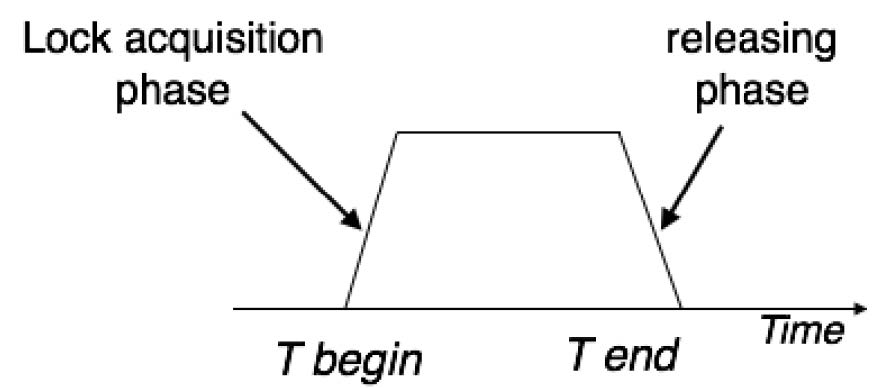
\includegraphics[width=0.8\textwidth]{Images/Two-phase locking.jpg}
  \caption{Two-phase locking}
\end{figure}

Two-Phase Locking (2PL) is a concurrency control method that guarantees
conflict-serializability. In this protocol, each transaction handles its
locks in two distinct and consecutive phases:

\begin{enumerate}
\item
  \textbf{Expanding phase (or Growing phase or Lock acquisition
  phase):}~In this first phase, the transaction acquires all the locks
  it needs. During this phase, no locks can be released.
\item
  \textbf{Shrinking phase (or Contracting phase or Releasing phase):}~In
  this second phase, the transaction releases its locks. During this
  phase, no new locks can be acquired.
\end{enumerate}

The fundamental rule of 2PL is that~\textbf{a transaction cannot acquire
any new locks after it has released a lock} (The rule refers to the
shrinking phase). In practice, this protocol is often implemented by
having a transaction acquire all necessary locks during its execution
(the growing phase) and then release all of them in a single operation
only after the~\texttt{commit}~or~\texttt{abort}~command has been
processed (the shrinking phase). Adherence to this protocol ensures that
the execution schedule of concurrent transactions is serializable,
thereby upholding the isolation property.

\subsubsection{Deadlocks}

A~\textbf{deadlock} is a situation where two or more transactions are in
a state of mutual waiting, where each transaction is blocked waiting for
a resource held by another transaction in the group. This creates a
circular dependency that can halt progress indefinitely.

Consider two transactions, T1 and T2:

\begin{itemize}
\item
  \texttt{T1:}~requests~\texttt{x\_lock(x)}~and then
  requests~\texttt{x\_lock(y)}
\item
  \texttt{T2:}~requests~\texttt{x\_lock(y)}~and then
  requests~\texttt{x\_lock(x)}
\end{itemize}

If T1 successfully acquires a lock on \texttt{x} and T2 simultaneously
acquires a lock on \texttt{y}, a deadlock occurs. T1 cannot proceed
because it is waiting for \texttt{y} (held by T2), and T2 cannot proceed
because it is waiting for \texttt{x} (held by T1).

For a deadlock to occur, four conditions (known as the Havender
conditions) must be met simultaneously:

\begin{enumerate}
\item
  \textbf{Mutual Exclusion:}~At least one resource must be held in a
  non-shareable mode.
\item
  \textbf{Incremental Accumulation (Hold and Wait):}~A transaction must
  be holding at least one resource while waiting to acquire additional
  resources held by other transactions.
\item
  \textbf{No Preemption:}~Resources cannot be forcibly taken from a
  transaction; they can only be released voluntarily by the transaction
  holding them.
\item
  \textbf{Circular Wait:}~A set of waiting transactions exists such that
  T1 is waiting for a resource held by T2, T2 is waiting for T3, and so
  on, with the final transaction in the chain waiting for a resource
  held by T1.
\end{enumerate}

Systems employ several strategies to manage deadlocks:

\begin{itemize}
\item
  \textbf{Prevention:}~Designing the system to annul one of the four
  necessary conditions. For example, requiring transactions to request
  all locks at once eliminates the "hold and wait" condition.
\item
  \textbf{Avoidance:}~Using algorithms, such as the
  Banker\textquotesingle s Algorithm, to analyze resource allocation
  requests and ensure the system never enters an unsafe state that could
  lead to a deadlock.

  The Banker\textquotesingle s algorithm is~a resource allocation and
  deadlock avoidance method that prevents a system from entering a
  "deadlocked" state by ensuring all processes can eventually complete.
  It works by simulating resource allocation to check if a request will
  lead to a "safe state," where a safe sequence of execution exists for
  all processes. If a request leads to an "unsafe state," the system
  denies the request, forcing the process to wait until resources are
  released.
\item
  \textbf{Detection and Resolution:}~Allowing deadlocks to occur,
  detecting them by building a wait-for graph to find cycles, and then
  resolving the deadlock by aborting one or more of the involved
  transactions.
\item
  \textbf{Timeouts:}~A simple but less precise strategy where a
  transaction aborts if a lock request is not granted within a specified
  time period. This risks aborting transactions that are not actually
  deadlocked.
\end{itemize}

The principles discussed so far primarily concern single-system
transactions. The next section shifts focus to the additional
complexities introduced when transactions must span multiple nodes in a
distributed environment.

\chapter{Transaction Processing in Distributed Systems}

Modern information systems frequently distribute data and processing
across multiple interconnected nodes to enhance performance,
scalability, and reliability. This architecture necessitates distributed
transactions, where a single logical transaction involves operations on
several distinct nodes. This section analyzes the rationale for
distributed transactions and their specific impact on the ACID
properties.

\section{Rationale and Impact on ACID Properties}

Distributed transactional systems are designed to achieve several key
goals:

\begin{itemize}
\item
  \textbf{Increase throughput}~by enabling parallelism, allowing
  different parts of a transaction or different transactions to execute
  on separate nodes simultaneously.
\item
  \textbf{Increase data availability and reliability}~by leveraging
  redundancy, where data is replicated across multiple nodes so that the
  failure of one node does not halt the entire system.
\end{itemize}

While distribution offers significant advantages, it introduces new
challenges for maintaining transactional integrity. The impact on the
ACID properties is not uniform:

\begin{itemize}
\item
  \textbf{Consistency}~and~\textbf{Durability}~remain the local
  responsibility of each participating node. Consistency depends on the
  correct implementation of operations on a given node, and durability
  relies on that node\textquotesingle s ability to write to stable
  storage.
\item
  \textbf{Isolation}~and~\textbf{Atomicity}, however, are significantly
  impacted. Ensuring that transactions are isolated from one another
  globally and that a transaction either commits or aborts
  across~\emph{all}~participating nodes requires specialized distributed
  protocols.
\end{itemize}

\section{Consistency in the Context of Data Redundancy}

A common question arises regarding the relationship between consistency
and data redundancy. Redundancy, which involves replicating data across
multiple nodes, is a powerful technique for improving availability and
fault tolerance. If one node containing a piece of data fails, other
nodes with replicas of that data can continue to service requests.

However, this redundancy places a new burden on
the~\textbf{Consistency}~property. In a system with redundant data,
consistency mandates that a transaction updating a piece of data must
ensure that the update is successfully propagated to~\textbf{all of its
replicas}. The system is in a consistent state only when all copies of a
data item are identical. If a transaction successfully updates the data
on one node but fails to update a replica on another, the system enters
an inconsistent state.

Distributed protocols like the Two-Phase Commit are designed to enforce
this global "all-or-nothing" outcome. By
guaranteeing~\textbf{distributed atomicity}, 2PC directly
upholds~\textbf{consistency}~across redundant data replicas, preventing
the system from entering a state where different nodes hold conflicting
versions of the same data.

\section{Distributed Transaction Protocols}

To solve the formidable challenges of maintaining atomicity and
isolation in a distributed context, systems employ specialized technical
protocols. These protocols coordinate actions across multiple nodes,
ensuring that global transactional properties are upheld despite network
uncertainties and node failures. This section details the methods for
distributed concurrency control and introduces the cornerstone protocol
for distributed atomicity: the Two-Phase Commit (2PC).

\subsection{Distributed Concurrency Control}

In a distributed transaction, the overall transaction is divided into
sub-transactions, each executed locally on a single node. Ensuring the
local serializability of these sub-transactions on each node is a
necessary but insufficient condition for guaranteeing global transaction
serializability.

Global serializability can be achieved if two conditions are met:

\begin{enumerate}
    \item
    Each participating node applies the \textbf{Two-Phase Locking
    (2PL)} protocol for its local sub-transactions.

    \item
    All sub-transactions commit \textbf{atomically} as a single unit.
\end{enumerate}

Managing~\textbf{distributed deadlocks}~also becomes more complex.
Building a global wait-for graph by combining information from all
participating nodes is difficult and often inefficient due to network
latencies and the potential for messages to be lost or delayed. For this
reason, using~\textbf{timeouts}~is a simpler and more common solution
for handling deadlocks in distributed systems.

\subsection{Distributed Reliability Control: The Two-Phase Commit (2PC) Protocol}

\begin{figure}
  \centering
  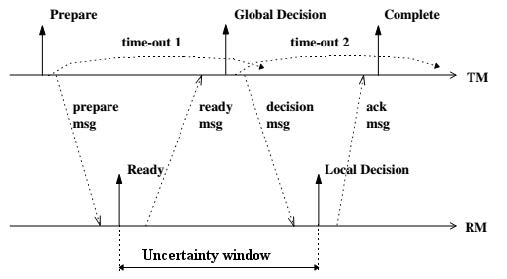
\includegraphics[width=\textwidth]{Images/Two-phase commit.jpg}
  \caption{Two-phase commit}
\end{figure}

The \textbf{Two-Phase Commit (2PC)} protocol is the standard industry
solution for guaranteeing distributed transaction atomicity. Its purpose
is to ensure that all participating nodes in a distributed transaction
reach the same final decision: either all of them commit their work, or
all of them abort.

The protocol defines two roles for participating nodes:

\begin{itemize}
\item
  \textbf{Transaction Manager (TM):}~A coordinator, with one TM per
  distributed transaction. The TM is responsible for initiating the
  protocol and making the final global commit or abort decision.
\item
  \textbf{Resource Manager (RM):}~A participant, with one RM for each
  node involved in the transaction. Each RM manages its local resources
  and votes on whether it can commit its sub-transaction.
\end{itemize}

2PC is a fault-tolerant protocol that relies on both message passing
between the TM and RMs and the writing of progress records to local logs
on each node. This logging ensures that the state of the transaction can
be recovered even if a node crashes.

\subsubsection{Protocol Flow: The Two Phases}

The protocol unfolds in two distinct phases: the voting phase and the
decision phase.

\paragraph{Phase 1: The Voting Phase}

\begin{enumerate}
\item
  The TM begins by writing a~\texttt{prepare}~record to its log and
  sends a~\texttt{prepare}~message to every RM.
\item
  Upon receiving the~\texttt{prepare}~message, each RM determines if it
  can reliably commit its sub-transaction. If it can, it writes
  a~\texttt{ready}~record to its local log and sends
  a~\texttt{ready}~message back to the TM. If it cannot commit, it
  immediately replies with a~\texttt{not-ready}~message.
\item
  The TM collects replies from all RMs. If it
  receives~\texttt{ready}~from every RM, it logs
  a~\texttt{global\ commit}. If it receives even
  one~\texttt{not-ready}~message or if a timeout occurs, the TM logs
  a~\texttt{global\ abort}.
\end{enumerate}

\paragraph{Phase 2: The Decision Phase}

\begin{enumerate}
\item
  The TM sends its final decision (\texttt{commit}~or~\texttt{abort}) in
  a message to all participating RMs.
\item
  Each RM receives the decision, writes the
  corresponding~\texttt{commit}~or~\texttt{abort}~record to its local
  log, performs the required action, and sends an acknowledgment
  (\texttt{ack}) message back to the TM.
\item
  Once the TM has received an~\texttt{ack}~from every RM, it knows that
  the decision has been uniformly enacted. It writes a
  final~\texttt{complete}~record to its log, marking the end of the
  distributed transaction.
\end{enumerate}

\subsubsection{Fault Handling and Considerations}

The 2PC protocol is designed to handle faults, with recovery based on
the last record found in the log of a failed node.

The most critical state for an RM is the~\textbf{uncertainty window}:
the period after it has sent its~\texttt{ready}~vote but before it has
received the TM\textquotesingle s final decision. This state is critical
because the RM has locked its local resources and cannot unilaterally
decide whether to commit or abort. It is blocked and must wait for the
TM to recover and provide the final outcome, potentially holding
critical resources and blocking other transactions indefinitely.

The Two-Phase Commit protocol has several important characteristics. It
is a~\textbf{blocking}~protocol, as RMs may have to wait for the TM to
make a decision. It is also~\textbf{resource-consuming}, requiring
multiple rounds of messaging and synchronous log writes. Furthermore,
the Transaction Manager can become a performance bottleneck or a single
point of failure. To mitigate some of these drawbacks, optimizations
such as "Presumed Abort" have been developed to reduce the amount of
logging and messaging required.

\chapter{Fault Tolerance and Consensus in Distributed Systems}

\section{Introduction to Faults in Distributed Systems}

The defining characteristic of a distributed system is its composition
of multiple, independent components that communicate over a network. The
overall reliability of such a system hinges on its ability to function
correctly despite the inevitable failure of some of these individual
components. To design systems that are resilient, robust, and
dependable, we must first understand the nature of these failures, or
"faults." A formal characterization of potential faults is the
foundational step in engineering systems that can tolerate them and
continue to provide correct service.

In the context of distributed systems, a \textbf{fault} is a condition
that may cause a component to deviate from its specified behavior. A
comprehensive taxonomy helps classify faults along several dimensions,
providing a structured way to reason about them.

\begin{itemize}
\item
  \textbf{Based on Phase of Creation:}

  \begin{itemize}
  \item
    \textbf{Development Faults:} These are errors introduced during the
    design or implementation phase, such as a bug in the code. An
    increasingly significant vector for this type of fault involves
    attacks on the software supply chain, where malicious code is
    inserted into shared libraries or repositories.
  \item
    \textbf{Operational Faults:} These faults manifest while the system
    is running, such as a hardware failure or a network outage.
  \end{itemize}
\item
  \textbf{Based on System Boundaries:}

  \begin{itemize}
  \item
    \textbf{Internal Faults:} Faults that occur within the nodes of the
    distributed system itself, such as a software crash on a
    participating server.
  \item
    \textbf{External Faults:} Faults that originate outside the
    system\textquotesingle s direct control, such as the failure of a
    connecting network or a dependency on a third-party service that
    becomes unavailable.
  \end{itemize}
\item
  \textbf{Based on Cause:}

  \begin{itemize}
  \item
    \textbf{Natural Faults:} Failures caused by environmental factors,
    like a natural disaster or an electricity outage.
  \item
    \textbf{Human-Made Faults:} Errors originating from human action,
    such as an error in a configuration update.
  \end{itemize}
\item
  \textbf{Based on Dimension:}

  \begin{itemize}
  \item
    \textbf{Hardware Faults:} Failures of physical components, which are
    often easier to anticipate and mitigate through strategies like
    redundancy.
  \item
    \textbf{Software Faults:} These are typically more open-ended and
    can be more difficult to prevent, mitigate, and recover from
    completely.
  \end{itemize}
\item
  \textbf{Based on Objective:}

  \begin{itemize}
  \item
    \textbf{Malicious Faults:} Faults caused with the explicit goal of
    disrupting the system, as in a deliberate attack.
  \item
    \textbf{Non-Malicious Faults:} Faults that occur without harmful
    intent, such as an accidental misconfiguration.
  \end{itemize}
\item
  \textbf{Based on Intent:}

  \begin{itemize}
  \item
    \textbf{Deliberate Faults:} A fault that is caused intentionally.
    This often overlaps with malicious faults but can also include
    non-malicious actions.
  \item
    \textbf{Non-Deliberate Faults:} An unintentional fault, often
    resulting from a mistake or unforeseen interaction.
  \end{itemize}
\item
  \textbf{Based on Capability:}

  \begin{itemize}
  \item
    \textbf{Accidental Faults:} Errors that arise from unforeseen
    circumstances.
  \item
    \textbf{Incompetence-Based Faults:} Errors caused by a lack of skill
    or knowledge. As the famous Hanlon\textquotesingle s razor suggests:
    "Never attribute to malice that which is adequately explained by
    stupidity."
  \end{itemize}
\item
  \textbf{Based on Persistence:}

  \begin{itemize}
  \item
    \textbf{Permanent Faults:} Faults that do not resolve on their own
    and require intervention to fix, such as permanent data loss or
    damaged hardware.
  \item
    \textbf{Transient Faults:} Temporary faults that resolve themselves
    without specific remediation, such as a brief network packet loss.
  \end{itemize}
\end{itemize}

To formally reason about the impact of these faults, we use an
\textbf{adversary model}, which defines the capabilities of a potential
source of failure. This chapter will focus on two of the most important
models: the relatively simple \textbf{Fail-Stop} model and the far more
challenging \textbf{Byzantine} model. Understanding these models is
essential for tackling the fundamental problem they create in
distributed systems: achieving consensus.

\section{The Core Challenge: The Consensus Problem}

For a distributed system to function as a cohesive whole---whether to
commit a database transaction, replicate a state machine, or elect a
leader---its independent nodes must be able to agree on a single value
or state. This process of reaching a collective, binding agreement among
a group of processes is known as the \textbf{consensus problem}. It is a
fundamental challenge because it must be solved in an environment where
communication can be unreliable and some processes may fail.

Formally, the consensus problem requires a protocol that allows a set of
processes to agree on a single data value. Any correct consensus
protocol must satisfy three fundamental properties:

\begin{enumerate}
\item
  \textbf{Agreement:} Every correct process must agree on the same
  value. There can be no ambiguity or disagreement among the functioning
  nodes.
\item
  \textbf{Integrity and Validity:} The \textbf{Integrity} property
  states that if all correct processes proposed the same initial value
  \emph{v}, then any correct process must decide on \emph{v}. A stronger
  version of this property, often called \textbf{Validity}, states that
  if a correct process decides on a value \emph{v}, then \emph{v} must
  have been proposed by \emph{some} correct process. These properties
  prevent the system from agreeing on a trivial or fabricated value.
\item
  \textbf{Termination:} Eventually, every correct process decides on
  some value. The protocol cannot run indefinitely; it must guarantee
  that it will eventually produce a result.
\end{enumerate}

The difficulty of this problem is underscored by the famous \textbf{FLP
impossibility theorem} (named for Fischer, Lynch, and Paterson). Its
core implication is that in a fully asynchronous system where
communication delays are unbounded, no deterministic algorithm can
guarantee that it will solve the consensus problem in a finite amount of
time if even a single process might fail by crashing. \\

For example, let us consider the Byzantine generals problem that we will discuss more in detail in the following sections (illustrated in figure 6.1):

\begin{figure}
  \centering
  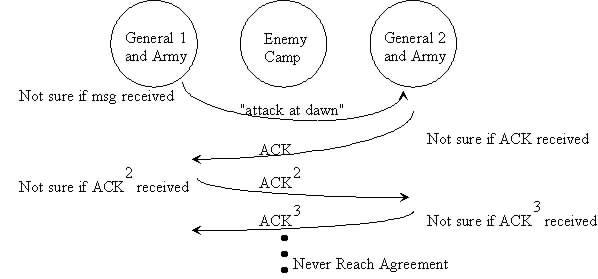
\includegraphics[width=\textwidth]{Images/Byzantine generals problem.jpg}
  \caption{Byzantine generals problem}
\end{figure}

Two generals must coordinate to attack the enemy with their armies at
the same time. Messengers must cross the enemy's camp to deliver the
message to the other general. Whenever a general sends a messenger they
cannot know if they will successfully deliver the message or not (maybe
because they get captured by the enemy). One might think that sending a
messenger with an acknowledgment message will solve the problem but it
doesn\textquotesingle t because the messenger responsible to deliver the
acknowledgment is in the exact same condition as the messenger with the
attack message. This means that the general sending the acknowledgment
needs another acknowledgment message from the other general that
confirms the successful reception of their acknowledgment message. This
creates an endless loop and an unsolvable problem! The process will
never terminate with all nodes agreeing on the same value.

The limit described by the FLP impossibility theorem forces designers to
either relax the asynchrony assumption or employ non-deterministic
(randomized) algorithms. To build practical solutions, we must first
precisely define the types of failures our system is designed to
withstand, which brings us to the formal adversary models.

\section{Adversary Models and Fault Tolerance}

To build fault-tolerant systems, we must first precisely define the
capabilities of a potential adversary. This is not limited to malicious
human actors; an "adversary" can represent any source of faults,
including hardware failures or software bugs. By formalizing the types
of behavior faulty components can exhibit, we can design and prove the
correctness of algorithms that tolerate them. The Fail-Stop and
Byzantine models represent two distinct and progressively more difficult
classes of failures to handle.

\subsection{The Fail-Stop Model and Crash Fault Tolerance}

The \textbf{Fail-Stop adversary model} represents the simplest and most
constrained type of failure. In this model, the adversary is only
capable of crashing a node. A faulty node can only fail in one way: it
abruptly stops all processing and communication. It does not send
incorrect data, corrupt messages, or exhibit any other malicious or
arbitrary behavior. From the perspective of other nodes, a fail-stop
node simply becomes unresponsive.

A system that can continue to operate correctly and maintain consensus
despite a certain number of its nodes experiencing fail-stop faults is
said to possess \textbf{Crash Fault Tolerance (CFT)}.

\subsection{The Byzantine Model and Byzantine Fault Tolerance}

The \textbf{Byzantine adversary model} represents the most challenging
class of failures. In this model, an adversary can completely control a
faulty node, forcing it to behave in any arbitrary and unpredictable
way. A Byzantine failure is a superset of a fail-stop failure---a
Byzantine node can always choose to simply crash---making it the most
general and difficult failure model to handle. A Byzantine node can:

\begin{itemize}
\item
  Send conflicting messages to different nodes (e.g., telling one peer
  to "attack" and another to "retreat").
\item
  Appear to be a functioning, correct node to a subset of observers
  while sending malicious data to others.
\item
  Delay or forge messages.
\item
  Remain silent for long periods and then suddenly resume activity with
  unpredictable behavior.
\end{itemize}

A system that can continue to operate correctly and achieve consensus
despite a certain number of its nodes being controlled by a Byzantine
adversary is said to possess \textbf{Byzantine Fault Tolerance (BFT)}.
Achieving BFT is exceptionally difficult because the protocol must be
resilient against an adversary with complete control over faulty nodes,
making no assumptions about their behavior.

Having defined these models, we can now analyze the mathematical limits
that govern how many faults of each type a system can tolerate.

\section{Analysis of Fault Tolerance Limits}

It is critically important to understand the theoretical limits of fault
tolerance. Before designing any consensus protocol, we must know what is
mathematically possible. Formal proofs establish the maximum number of
faulty nodes (\texttt{f}) that a system with a total number of nodes
(\texttt{N}) can withstand and still guarantee the properties of
consensus (Agreement, Integrity, and Termination). This section will
demonstrate these fundamental limits for both the Fail-Stop and
Byzantine models.

\subsection{Maximum Tolerable Faults in the Fail-Stop Model}

For a system to be crash-fault tolerant, the maximum number of nodes
that can fail is strictly less than half of the total nodes.

\textbf{Formal Limit:} A system can tolerate a maximum of \texttt{f}
crash faults only if $f < N/2$.

This limit can be demonstrated logically through the concept of a
\textbf{quorum}, or a majority. For a distributed system to make an
unambiguous decision and make progress, the set of active, correct nodes
must constitute a strict majority of the total.

Consider the scenario where this condition is violated, and
$f \geq N/2$. The number of remaining active nodes would be
$N - f$. Since $f \geq N/2$, it follows that
$N-f \leq N/2$. In this state, the remaining active nodes
represent half or less than half of the original system. They can no
longer form a decisive majority. This can lead to two critical problems:

\begin{enumerate}
\item
  \textbf{Network Partition (Split-Brain):} The active nodes might be
  unable to distinguish whether the other nodes have crashed or if they
  themselves have been partitioned from the network. Without a majority,
  two separate partitions could potentially make conflicting decisions,
  violating the Agreement property.
\item
  \textbf{Inability to Make Progress:} If decisions require a majority
  vote to proceed, a system with half or fewer of its nodes active
  cannot achieve a quorum. The system would stall, violating the
  "Termination" property.
\end{enumerate}

Therefore, to guarantee correctness and progress, a system must always
be able to form a majority, which requires
$N - f > N/2$, or $f < N/2$.

\subsection{Maximum Tolerable Faults in the Byzantine Model}

For a system to be Byzantine-fault tolerant using "oral messages" (i.e.,
unauthenticated messages where the sender is known but the message
content can be forged), the number of faulty nodes must be strictly less
than one-third of the total nodes.

\textbf{Formal Limit:} A system can tolerate a maximum of $f$ Byzantine faults only if $f < N/3$, which is equivalent to requiring a total of $N \geq 3f + 1$ nodes.

It is crucial to note that this limit applies to systems without authenticated messages. Protocols that use unforgeable message signatures, such as those enabled by public-key cryptography, can
achieve BFT in the presence of an arbitrary number of faulty nodes.

The $f < N/3$ limit is classically analyzed using the \textbf{Byzantine Generals Problem}, an allegory where a group of generals must agree on a plan (attack or retreat) but some of them may
be traitors who will actively try to thwart the agreement. The generals represent nodes, and traitors represent Byzantine-faulty nodes.

First, let\textquotesingle s demonstrate the impossibility of a solution
for the specific case of $N=3$ generals with $f=1$
traitor. Imagine one Commander and two Lieutenants. The Commander issues an order, and the Lieutenants must agree on that order.

\begin{itemize}
\item
  \textbf{Case A: The Commander is a traitor.} The Commander sends
  "attack" to Lieutenant 1 and "retreat" to Lieutenant 2. Lieutenant 1
  tells Lieutenant 2, "The Commander said attack." Lieutenant 2 now has
  two conflicting messages: "retreat" (from the Commander) and "The
  Commander said attack" (from Lieutenant 1). Lieutenant 2 cannot
  determine whether the Commander is the traitor (for sending
  conflicting orders) or if Lieutenant 1 is the traitor (for lying about
  the Commander\textquotesingle s order).
\item
  \textbf{Case B: A Lieutenant is a traitor.} The Commander (who is
  loyal) sends "attack" to both Lieutenants. Lieutenant 1 (loyal)
  receives "attack". Lieutenant 2 (traitor) also receives "attack" but
  tells Lieutenant 1, "The Commander said retreat." From Lieutenant
  1\textquotesingle s perspective, this is identical to the situation in
  Case A. He has received "attack" from the Commander and "retreat" from
  his peer. He cannot distinguish between a traitorous Commander and a
  traitorous Lieutenant.
\end{itemize}

Because a loyal lieutenant cannot resolve this ambiguity, it is impossible to guarantee consensus. Thus, no solution exists for $N=3$, $f=1$.

The general proof for $f \geq N/3$ works by reduction. It states that if a
solution existed for \emph{any} system where $f \geq N/3$, one could use that hypothetical solution to solve the $N=3$ and $f=1$ case, which we just demonstrated is unsolvable. This logical contradiction proves that no general solution can exist for $f \geq N/3$. Therefore, any BFT protocol using oral messages must operate with $N \geq 3f + 1$ nodes.

With these theoretical boundaries established, we can now examine the
algorithms designed to achieve consensus within these limits.

\section{Algorithms for Achieving Consensus}

Now that the theoretical boundaries of fault tolerance are understood,
this section explores concrete algorithms that provide fault tolerance
within those established limits. These algorithms offer constructive
methods for achieving consensus in the face of Fail-Stop and Byzantine
faults.

\subsection{Atomic Broadcast: Consensus on a Sequence}

In the formal literature of distributed systems, the term
\textbf{consensus} typically refers to an agreement on a single event or
value. However, many real-world systems, especially those implementing
state machine replication, need to agree on a totally ordered
\emph{sequence} of operations or messages. This more specific problem is
known as \textbf{Atomic Broadcast}. An atomic broadcast protocol ensures
that all correct nodes deliver the same sequence of messages to their
local applications.

An Atomic Broadcast protocol must possess the following four properties:

\begin{itemize}
\item
  \textbf{Validity:} If a correct node broadcasts a message \texttt{m},
  then that node eventually delivers \texttt{m}.
\item
  \textbf{Agreement:} If a message \texttt{m} is delivered by some
  correct node, then \texttt{m} is eventually delivered by every correct
  node.
\item
  \textbf{Integrity:} No correct node delivers the same message more
  than once. Furthermore, if a correct node delivers a message
  \texttt{m} from a correct sender \texttt{p}, then \texttt{m} was
  previously broadcast by \texttt{p}.
\item
  \textbf{Total Order:} For any two messages \texttt{m1} and
  \texttt{m2}, if two correct nodes \texttt{p} and \texttt{q} both
  deliver them, then \texttt{p} delivers \texttt{m1} before \texttt{m2}
  if and only if \texttt{q} delivers \texttt{m1} before \texttt{m2}.
  This ensures all nodes process messages in the exact same sequence.
\end{itemize}

Protocols such as \textbf{Paxos} and \textbf{Viewstamped Replication
(VSR)} are notable examples of algorithms that provide Atomic Broadcast.
They are proven to be crash-fault tolerant, operating correctly as long
as the number of failures \texttt{f} is less than \texttt{N/2}.

\subsection{The Oral Message Algorithm for Byzantine Agreement}

The \textbf{Oral Message (OM) algorithm} is a constructive, recursive
algorithm that solves the Byzantine Generals Problem, providing a
solution for Byzantine agreement in systems where
$N \geq 3f + 1$. The core idea is that nodes reach a decision
based on a majority of the messages they receive, with a recursive
structure to filter out the lies of traitors.

The algorithm, \texttt{OM(m)}, is designed to tolerate up to \texttt{m}
traitors.

\begin{itemize}
\item
  \textbf{Base Case: OM(0)} (tolerating zero traitors)

  \begin{enumerate}
  \item
    The Commander sends an order to every Lieutenant.
  \item
    Each Lieutenant follows the order received. If no order is received,
    they use a default value (e.g., RETREAT).
  \end{enumerate}
\item
  \textbf{Recursive Step: OM(m) where m \textgreater{} 0} (tolerating
  \texttt{m} traitors)

  \begin{enumerate}
  \item
    The Commander sends an order to every Lieutenant.
  \item
    Each Lieutenant \texttt{i} receives a value \texttt{vi} from the
    Commander. Lieutenant \texttt{i} then acts as the commander in a new
    instance of the algorithm, \texttt{OM(m-1)}, to send the value
    \texttt{vi} to all \emph{other} \texttt{N-2} Lieutenants.
  \item
    Each Lieutenant \texttt{i} collects all the values it received from
    the other lieutenants in step 2. It then uses the \textbf{majority}
    of all received values (including the one from the original
    Commander) as its final decision.
  \end{enumerate}
\end{itemize}

Let\textquotesingle s illustrate the algorithm\textquotesingle s
effectiveness in the case of \texttt{N=4} and \texttt{f=1}
(\texttt{m=1}):

\subsubsection{Scenario 1: Traitor Lieutenant}

\begin{figure}
  \centering
  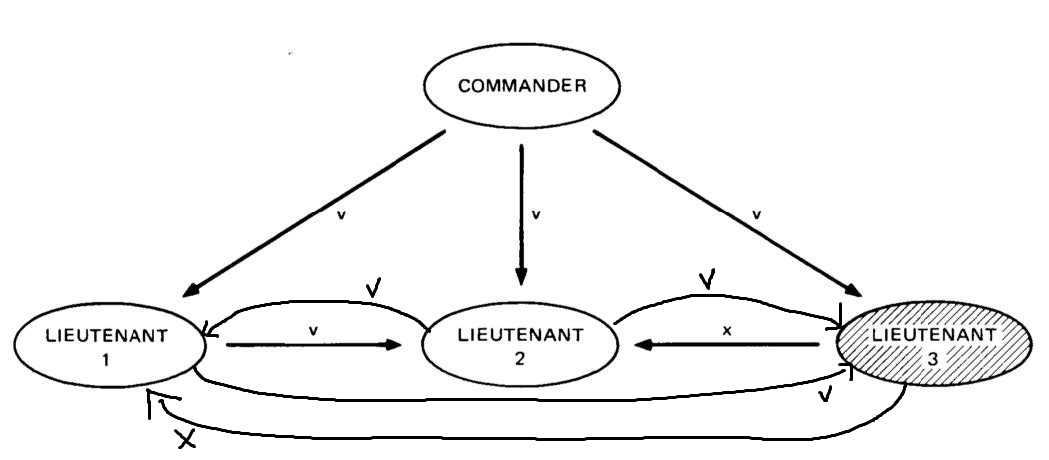
\includegraphics[width=\textwidth]{Images/Traitor lieutenant.jpg}
  \caption{Traitor lieutenant}
\end{figure}

The Commander is loyal and sends "attack" (`v`) to all three Lieutenants
(L1, L2, L3). L1 and L2 are loyal, but L3 is a traitor. In the recursive
step, L1 and L2 will correctly relay `v` to each other. The traitor, L3,
might send a false value, "retreat" (`x`), to L2.

Lieutenant L2 will have received three values:

\begin{enumerate}
\item
  \texttt{v} from the Commander.
\item
  \texttt{v} relayed from the loyal L1.
\item
  \texttt{x} relayed from the traitor L3.
\end{enumerate}

By applying the majority function to \texttt{\{v,\ v,\ x\}}, L2
correctly decides on \texttt{v} ("attack"). The same logic applies to
L1, and thus all loyal lieutenants reach the correct consensus.

\subsubsection{Scenario 2: Traitor Commander}

\begin{figure}
  \centering
  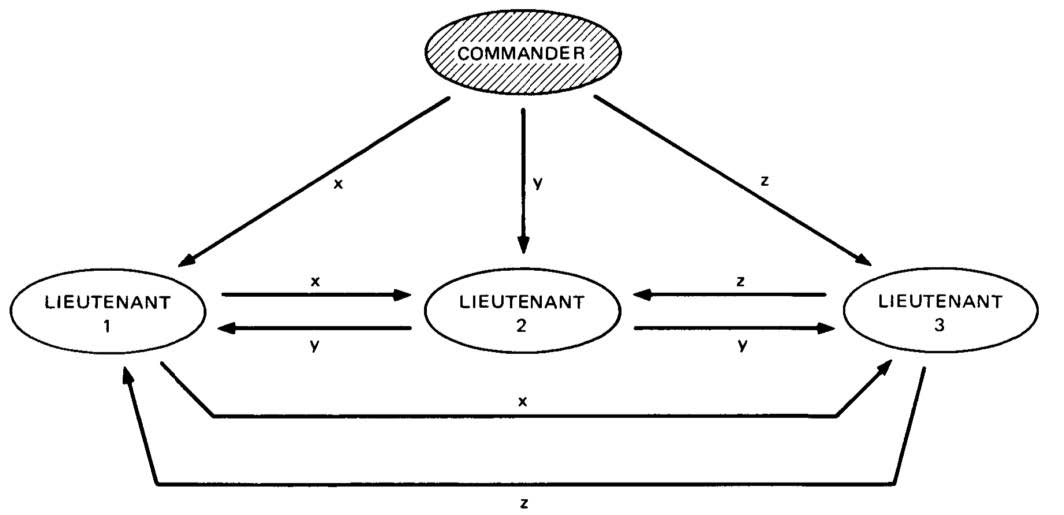
\includegraphics[width=\textwidth]{Images/Traitor commander.jpg}
  \caption{Traitor commander}
\end{figure}

The Commander is a traitor and sends conflicting orders: "attack" (`x`)
to L1, "retreat" (`y`) to L2, and "attack" (`z`) to L3. All Lieutenants
are loyal. In the recursive step, they will faithfully relay the orders
they received to each other.

For example, Lieutenant L1 will end up with three values:

\begin{enumerate}
\item
  \texttt{x} from the traitor Commander.
\item
  \texttt{y} relayed from L2.
\item
  \texttt{z} relayed from L3.
\end{enumerate}

All other loyal lieutenants will also end up with the set of values
\texttt{\{x,\ y,\ z\}}. Because there is no majority, they must use a
default, pre-agreed rule to break the tie (e.g., choosing the
lexicographically first value or a default like "retreat"). Since all
loyal lieutenants have the same set of values and apply the same rule,
they are guaranteed to reach the same decision, satisfying the Agreement
property even with a traitorous commander.

While correct, the Oral Message algorithm is highly inefficient. Its
message complexity grows exponentially with the number of faults to be
tolerated, making it prohibitively expensive for most practical
applications. This has led to the development of more optimized BFT
protocols.

\subsection{Real-World Applications of Fault Tolerance}

The theoretical concepts of Crash Fault Tolerance (CFT) and Byzantine
Fault Tolerance (BFT) are not merely academic exercises; they form the
bedrock of some of the most critical and innovative distributed systems
in operation today. From ensuring the safety of air travel to securing
billions of dollars in digital assets, these principles are essential
for building trustworthy applications in a decentralized world.

\begin{itemize}
\item
  \textbf{Blockchain and Cryptocurrencies:} Systems like Bitcoin use
  consensus mechanisms, such as Proof-of-Work, as a large-scale,
  practical solution to the Byzantine Generals Problem. This enables a
  global, trustless network of anonymous participants to agree on a
  single, shared ledger of transactions. BFT is the core property that
  secures the network against malicious actors attempting to
  double-spend coins or rewrite history, establishing trust not in
  individual participants, but in the protocol itself.
\item
  \textbf{Aerospace and Aviation:} The flight control systems of modern
  aircraft, including the Boeing 777 and 787, employ Byzantine Fault
  Tolerance to achieve extreme reliability and safety. In these
  "fly-by-wire" systems, multiple redundant computers process pilot
  inputs and sensor data. BFT protocols ensure that the computers can
  reach a correct consensus on control actions even if one component
  suffers a hardware or software fault that causes it to behave
  erratically. This guarantees the aircraft remains controllable under
  the most severe failure conditions.
\item
  \textbf{Cloud Computing and Distributed Databases:} Large-scale cloud
  services and distributed databases rely heavily on crash-fault
  tolerant consensus protocols (like Paxos and Raft) to manage critical
  operations. These algorithms are used to reliably replicate data
  across multiple servers and data centers, elect a single leader for a
  cluster of nodes, and atomically commit distributed transactions. This
  ensures the high availability and data integrity that customers expect
  from cloud infrastructure, preventing data loss even if entire servers
  or data centers fail.
\end{itemize}

As our technological infrastructure becomes ever more distributed and
decentralized, the principles of fault tolerance and consensus are no
longer niche concerns but fundamental engineering requirements. Building
robust, secure, and trustworthy applications for the future depends
directly on a solid understanding of how to make systems work correctly,
even when parts of them fail.

\end{document}
